\documentclass[12pt, twoside, openany]{report}
\usepackage[dvips]{graphicx,color,rotating}
\usepackage[utf8]{inputenc}
\usepackage{indentfirst}
\usepackage{t1enc}
\usepackage{a4wide}
\usepackage{amsfonts}
\usepackage{amsmath}
\usepackage{caption}
\usepackage{enumerate}
\usepackage{verbatim}
\usepackage[MeX]{polski}
\usepackage[T1]{fontenc}
\usepackage{geometry}
\geometry{left=25mm,right=25mm,bindingoffset=10mm, top=25mm, bottom=25mm}
\usepackage{amssymb, latexsym}
\usepackage{amsthm}
\usepackage{palatino}
\usepackage{float}
\usepackage{tabulary}
\usepackage{array}
\usepackage{pstricks}
\usepackage{textcomp}
\usepackage{url}
\usepackage{listings}
\usepackage{xcolor}
\usepackage{courier}
\usepackage{pgfplots}
\usepackage{etoolbox}
\patchcmd{\abstract}{\null\vfil}{}{}{} % abstract top align.

\newtheorem{twierdzenie}{Twierdzenie}[section]

%\linespread{1.5}

% styl listingów
\lstset{
    xleftmargin=17pt,
    numbers = left,
    %framexleftmargin=10mm,
    frame=lrbt,
    %backgroundcolor=\color[RGB]{250,250,250},
    %keywordstyle=\bfseries\color{blue},
    %identifierstyle=\bfseries,
    %numberstyle=\color[RGB]{0,192,192},
    %commentstyle=\it\color[RGB]{96,96,96},
    %stringstyle=\rmfamily\slshape\color[RGB]{128,0,0},
    %showstringspaces=true,
    breaklines=true,
    breakatwhitespace=try,
    %language=C++,
    showstringspaces=false,
    tabsize=4,
    basicstyle=\footnotesize\ttfamily,
    aboveskip=1em
    %postbreak=\raisebox{0ex}[0ex][0ex]{\ensuremath{\color{red}\hookrightarrow\space}}
}


\author{Mateusz Bartkowiak}
\title{Współbieżne modelowanie i~prezentacja dynamiki obiektów fizycznych}


\begin{document}

\begin{titlepage}

\noindent


\centering
\Large POLITECHNIKA POZNAŃSKA\\
\large WYDZIAŁ ELEKTRYCZNY\\
Instytut Automatyki i Inżynierii Informatycznej
\vfill
\includegraphics[width=120pt,height=120pt]{PP}

\vfill
\center
\LARGE
Mateusz Bartkowiak

\center
\Large
Praca inżynierska

\vfill
\center
\Huge
\textbf{Współbieżne modelowanie i~prezentacja dynamiki obiektów fizycznych}


\vfill
\center
\Large
Promotor: dr inż. Andrzej Sikorski

\vfill
\center
\large
Poznań, styczeń 2017

\end{titlepage}

% wlasny abstract
\renewcommand{\abstractname}{}
\begin{abstract}
\thispagestyle{plain} % numer strony
\begin{center}
\textbf{Streszczenie}
\end{center}

\indent Przedmiotem niniejszej pracy jest implementacja symulatora n ciał. Polega ona na zaprogramowaniu układu ruchomych punktów materialnych w przestrzeni trójwymiarowej, które oddziałują na siebie siłą grawitacji. Istotnym elementem pracy jest zrównoleglenie kluczowych dla wydajności symulatora obliczeń oraz prezentacja przebiegu symulacji na trójwymiarowej scenie w czasie rzeczywistym. Korzyści z~zastosowania wielowątkowości zbadane zostały pod kątem płynności wyświetlanej animacji. Przedstawiono również implikację parametrów wejściowych na przebieg symulacji.

\vspace{50px}
\begin{center}
\textbf{Abstract}
\end{center}

\indent
The subject of the following work is the implementation of the n-body simulator. This involves programming of the moving material points in three-dimensional space, interacting under the influence of gravitational forces. The key contribution of this work is parallelisation of the computationally expensive routines which are the key to achieving real-time simulations. The proposed multithreaded implementation was examined in terms of frame rate. The influence of particular input parameters on the simulation itself was also assessed as a part of this thesis.

\end{abstract}


\tableofcontents


%-----------Poczatek czesci zasadniczej-----------

\chapter{Wstęp}

Symulacje komputerowe pozwalają na predykcje zachowywania się określonych obiektów w~zamodelowanym środowisku. Odtwarzanie określonych zjawisk fizycznych możliwe jest dzięki zastosowaniu odpowiednich metod numerycznych. Pozwalają one na uzyskanie wyników, które z reguły są tylko przybliżeniem świata rzeczywistego. Dokładność symulacji często może być poprawiana poprzez uwzględnianie kolejnych czynników, co z kolei zwiększa kosztowność obliczeń. Jednakże dobierając odpowiednie metody, algorytmy czy podejścia do obliczeń, można znacząco zwiększyć wydajność pracy symulatora. Istotnym zagadnieniem jest również sposób prezentacji uzyskanych wyników. Metoda przedstawienia efektów zależy w~głównej mierze od celu wykonywania symulacji i może przybierać wiele form.

\section{Cel pracy}

Celem pracy jest implementacja symulatora wielu ciał, wykorzystując wielowątkowość do obliczania dynamiki obiektów oraz grafikę trójwymiarową do prezentacji przebiegu symulacji. Na przykładzie tej implementacji można opisać kwestie będące motywem przewodnim pracy -- współbieżność obliczeń i prezentacja obiektów fizycznych.

Ciała reprezentowane są przez punkty materialne i oddziałują na siebie siłą grawitacji. Ponieważ obliczanie ruchu ciał przy dużej ich ilość zajmuje największy czas procesora, a ruch każdego ciała obliczany jest niezależnie od innych, naturalnym wydaje się więc zastosowanie wielowątkowości.

Oprócz optymalnego wykonania obliczeń, należy zapewnić odpowiednią prezentację działania symulatora. Dla problemu będącego tematem przewodnim pracy, najlepszym sposobem prezentacji, oprócz dostarczania pożądanych informacji liczbowych, jest zastosowanie grafiki trójwymiarowej. Dzięki niej można w czasie rzeczywistym śledzić ruch obiektów znajdujących się w zamodelowanym środowisku.

Ważnym aspektem pracy jest analiza wpływu parametrów wejściowych na przebieg symulacji i wydajność symulatora. Przebieg symulacji można badać, śledząc aktywność ciał, a wydajność mierzyć liczbą klatek na sekundę.

Mnogość zagadnień z jakimi musi się zmierzyć programista motywuję do poszerzania swojej wiedzy i kompetencji. A umiejętności nabyte przy projektowaniu i~implementacji opisanego symulatora można wykorzystać w wielu dziedzinach pokrewnych.

\section{Omówienie rozdziałów}

Praca ta zaczyna się od przedstawienia problemu wielu ciał. Dalej wspomniane jest prawo powszechnego ciążenia w~kontekście obliczania sił działających między parą ciał, po czym opisane są sposoby wyznaczania sił wypadkowych działających na ciała. Następnie scharakteryzowane są podstawowe metody obliczeń numerycznych, które są odpowiedzialne za rozwiązywanie równań ruchu. Rozdział trzeci traktuje o przetwarzaniu równoległym na przykładzie biblioteki Intel Threading Building Blocks. W następnym rozdziale opisane są najważniejsze zagadnienia programowania grafiki trójwymiarowej, których zrozumienie jest niezbędne do implementacji symulatora wielu ciał. Rozdział ten rozpoczyna się od wyjaśnienia podstawowych zagadnień związanych z przestrzenią trójwymiarową i przekształceniami na układach współrzędnych, w~tym działanie potoku renderowania. Dalej opisana jest biblioteka OpenGL wraz z bibliotekami pomocniczymi. Następnie opisane są bufory w OpenGL, wierzchołki i~ich atrybuty oraz shadery wierzchołków i fragmentów. Dalej opisany jest projekt i implementacja symulatora, począwszy od koncepcji i wymienieniu wykorzystanych technologi, aż do omówienia wszystkich struktur i najważniejszych fragmentów programu. W przedostatnim rozdziale przedstawiony jest sposób użytkowania symulatora, jego działanie oraz omówienie przeprowadzonych na nim testów wydajności. Pracę kończy podsumowanie implementacji symulatora wielu ciał.

\chapter{Problem wielu ciał}

Problem wielu ciał jest zagadnieniem mechaniki klasycznej. Polega ono na wyznaczaniu toru ruchów ciał o danych masach, prędkościach i położeniach początkowych w danym układzie n ciał zakładając, że owe ciała oddziałują ze sobą zgodnie z prawem powszechnego ciążenia Newtona.

Symulacja zjawiska opartego na problemie wielu ciał ma zastosowanie głównie w astronomii, dynamice płynów, czy w dynamice molekularnej, w której bada się ruchy atomów i cząsteczek. Przykładem może być predykcja zwijania białka, w której ważnym elementem jest obliczenie oddziaływania międzycząsteczkowego van der Waals’a. Innym przykładem zastosowania symulacji wielu ciał jest symulacja przepływów turbulentnych cieczy i gazów \cite{bib:gpu_gems}.

\section{Wyznaczanie siły}
\label{wyznaczanie_sily}

Kluczowym elementem symulacji wielu ciał jest obliczanie siły oddziałującej na dane ciało w danej chwili. Aby obliczyć siłę z jaką oddziałują na siebie dwa ciała korzysta się z prawa powszechnego ciążenia Newtona brzmiącego: \textit{Między dowolną parą ciał posiadających masy pojawia się siła przyciągająca, która działa na linii łączącej ich środki, a jej wartość rośnie z iloczynem ich mas i maleje z kwadratem odległości}. Prawo te dane jest wzorem:

\begin{equation}
\label{eq:sila}
f_{ij}=G\frac{m_i m_j}{|r_{ij}|^2} \hat{r}_{ij}
\end{equation}
gdzie:

\indent $ f_{ij} $ -- siła z jaką ciało $j$ oddziałuje na ciało $i$,

\indent $ G $ -- stała grawitacji,

\indent $ m_{i} $ -- masa ciała $i$,

\indent $ m_{j} $ -- masa ciała $j$,

\indent $ |r_{ij}| $ -- odległość między środkami mas ciała $i$ oraz ciała $j$,

\indent $ \hat{r}_{ij} $ -- wersor wektora łączącego środki mas ciała $i$ oraz ciała $j$.

\bigskip


Sumując siły oddziaływania ciała $i$ z każdym innym ciałem układu $N$ ciał, otrzymujemy siłę wypadkową $F_i$ działającą na ciało $i$:

\begin{equation}
\label{eq:sila_wypadkowa}
F_i=Gm_i \times \sum\limits_{\substack{i\le j \le N \\ j \neq i}} \frac{m_j}{|r_{ij}|^2} \hat{r}_{ij}
\end{equation}

W praktyce oznacza to obliczenie sił między wszystkimi istniejącymi parami ciał w układzie $N$ ciał, co skutkuje złożonością obliczeniową $\mathcal{O}(n^2)$. Ponieważ wektor siły z jaką ciało $i$ oddziałuje na ciało $j$ ma przeciwny zwrot do wektora siły z jaką ciało $j$ oddziałuje na ciało $i$, wystarczy obliczyć siłę $f_{ij}$, a do siły $f_{ji}$ przypisać ujemną wartość $f_{ij}$. Dzięki temu redukujemy ilość obliczeń działających sił dwukrotnie. Dokładną liczbę $C$ par ciał, między którymi należy obliczyć działającą siłę, można wyznaczyć korzystając z kombinacji bez powtórzeń danej wzorem:

\begin{equation}
\label{eq:liczba_par}
C_2^N = \left(\begin{array}{c}N\\ 2\end{array}\right) = \frac {N!}{2(N-2)!}
\end{equation}

Istnieją algorytmy, które zmniejszają złożoność obliczeniową symulacji wielu ciał. Przykładem jest algorytm Barnes-Hut o złożoności $\mathcal{O}(n\log{}n)$. Jest to algorytm aproksymacyjny, co oznacza, że daje on przybliżone wyniki. Idea jego działania opiera się na dzieleniu przestrzeni, co pozwala na grupowanie sąsiednich ciał w jedno ciało o~masie równej sumie mas zgrupowanych ciał oraz środku leżącym w środku masy tych ciał.

\section{Dynamika punktu materialnego}

Ciało może być reprezentowane jest jako punkt materialny, czyli posiadające masę, lecz o nieskończenie małych rozmiarach. Do opisu ruchu ciała niezbędna jest wiedza o położeniach ciała w danych momentach czasowych. Ze względu na skończony i określony odstęp czasowy między momentami badania położenia ciała, ruch ten będzie tylko przybliżeniem. Nie jest to jednak istotne dla prostej symulacji, w~której wyniki prezentowane są na ekranie w postaci animacji.

W przypadku symulacji wielu ciał istotną role odgrywa związek między siłą a~przyspieszeniem, którą opisuje druga zasada dynamiki Newtona, mówiąca że \textit{wektor przyspieszenia $\overset{\text{\scriptsize$\rightarrow$}}{a}$ jest zawsze równoległy do wektora siły $\overset{\text{\scriptsize$\rightarrow$}}{F}$, a jego wartość jest proporcjonalna do wartości siły}. Zależność ta dana jest wzorem:

\begin{equation}
\label{eq:przyspieszenie}
\overset{\text{\scriptsize$\rightarrow$}}{a} = \frac{\overset{\text{\scriptsize$\rightarrow$}}{F}}{m}
\end{equation}


We wzorze tym współczynnikiem proporcjonalności między działającą siłą a spowodowanym przez nią przyspieszeniem jest masa $m$, ponieważ im jest ona większa, tym mniejszy efekt powoduje przyłożenie siły.

Ponieważ przyspieszenie ciała w każdej chwili czasu jest znane (wyznacza ja działająca na ciało siła), do wyznaczenia pozostaje zatem położenie i prędkość w kolejnych chwilach czasu. Sprowadza się to do rozwiązywania równań różniczkowych ruchu\footnote{Problem rozwiązywania równań ruchu należy do szerszej klasy tzw. zagadnień początkowych. Rozwiązywane są w nich równania różniczkowe zwyczajne względem czasu (lub innego parametru) znając rozwiązanie w chwili początkowej \cite{bib:dziubak}.}
odpowiednimi metodami numerycznymi. Jedną z nich jest prosty algorytm Eulera. Innym przykładem może być dokładniejszy algorytm Verleta, czy algorytm Runge-Kutty czwartego rzędu (RK4), który jest wolny, lecz jego dokładność pozwala na zwiększenie kroku czasowego.

Algorytm RK4 jest raczej stosowany w symulacjach, które nie są przeprowadzane w czasie rzeczywistym. Jednak w symulacjach przeprowadzanych na potrzeby grafiki trójwymiarowej dokładność obliczeń nie jest priorytetem, ponieważ różnice, które nie będą widoczne na ekranie, są bez znaczenia.

Algorytm Eulera sprawdza się zaskakująco dobrze w przypadku symulacji prostych układów, jak np. w grach. Wysoka precyzja nie jest wówczas priorytetem. Ponadto przyłożone do ciał siły są często kontrolowane przez gracza, co oznacza nagłe i częste zmiany ich wartości. Wpływ zmian siły będzie więc i tak dominował nad efektami utraty dokładności. Wyznaczenie tą metodą położenia $x$ w następnej chwili $t_0 + \triangle t$ opisuje wzór:

\begin{equation}
\label{eq:euler}
x(t_0 + \triangle t) \approx x(t_0) + \dot{x} (t_0) \triangle t + \ddot{x} (t_0) \triangle t^2
\end{equation}
gdzie:

\indent $ \dot{x} $ -- prędkość ciała,

\indent $ \ddot{x} $ -- przyspieszenie ciała,

\indent $ t_0 $ -- ostatnio badana chwila,

\indent $ \triangle t $ -- krok czasowy.

\bigskip

Algorytm Verleta jest łatwy do implementacji, dokładny i stabilny. Jego podstawową zaletą jest większa dokładność przy niewiele większym koszcie obliczeniowym w porównaniu z algorytmem Eulera. Położenie w następnej chwili metodą Verleta dane jest wzorem:

\begin{equation}
\label{eq:verlet}
x(t_0 + \triangle t) \approx -x(t_0 - \triangle t) + 2x(t_0) + \ddot{x} (t_0) \triangle t^2
\end{equation}

Wzór ten wiąże bezpośrednio położenie i przyspieszenie, a zatem algorytm nie generuje pierwszych pochodnych położenia (prędkości).
Należy jednak znać położenie kroku poprzedniego, dlatego w chwili zerowej można obliczyć następne położenie korzystając z algorytmu Eulera.

Stosując wymienione metody, długość kroku czasowego powinna być niewielka, ponieważ zakłada się, że przyspieszenie się nie zmienia i aktualizowane jest dopiero w następnym kroku czasowym.


\chapter{Przetwarzanie współbieżne}

Aby przyspieszyć wykonywanie się programu, można zrównoleglić obliczenia, które przeprowadzane są niezależnie od siebie. W przypadku procesora z paroma rdzeniami, zrównoleglenie najczęściej polega na zastosowaniu dodatkowych wątków. Wątki te mogą działać równocześnie, każdy na innym rdzeniu. Technika ta nosi nazwę przetwarzania współbieżnego i zastosowana została w niniejszej pracy przy użyciu opisanej w tym rozdziale biblioteki TBB (ang. \textit{Intel Threading Building Blocks}).

\section {Biblioteka Intel Threading Building Blocks}
\label{tbb}

TBB jest biblioteką firmy Intel napisaną w języku C++ służącą do programowania równoległego. Jest zoptymalizowana do działania na wszystkich architekturach procesorów Intel. Wspiera wiele systemów operacyjnych oraz nie wymaga specjalnego kompilatora. Biblioteka ta automatycznie zarządza wątkami zapewniając najefektywniejsze użycie zasobów procesora jednocześnie dostarczając wysokopoziomowe i proste rozwiązania w języku C++.
Biblioteka TBB w dużej części opiera się na paradygmacie programowania generycznego, zapewniając niezależność funkcjonalności od typów, algorytmów czy struktur danych.

\section{Dzielenie przestrzeni obliczeń}
\label{dzielenie_przestrzeni_obliczen}

Podstawową metodą zrównoleglenia obliczeń w bibliotece TBB jest funkcja \\\texttt{parallel\_for}, która dzieli przestrzeń obliczeń na mniejsze części i uruchamia je na osobnych wątkach. Można ją wykorzystać, aby przyspieszyć wykonywanie się funkcji pokazanej na listingu \ref{lst:tbb1}.

\lstinputlisting[caption={Przykładowa funkcja wykonująca obliczenia sekwencyjne \cite{bib:tbb}.}, captionpos=b, label={lst:tbb1}]{tbb1.cpp}

Pierwszym krokiem, aby przyspieszyć obliczenia jest obudowanie funkcji w klasę i przeciążenie operatora \texttt{()}, który będzie odpowiedzialny za przetwarzanie części zadania. Dzięki temu możliwe będzie wywołanie obiektu tak, jakby był on funkcją. Pokazane jest to na listingu \ref{lst:tbb2}.

\lstinputlisting[caption={Funkcja z listingu \ref{lst:tbb1} obudowana w klasę \cite{bib:tbb}.}, captionpos=b, label={lst:tbb2}]{tbb2.cpp}

Konstruktor klasy \texttt{ApplyFoo} ustawia pola obiektu. Operator \texttt{()} przypisuje zmienną \texttt{my\_a} do zmiennej lokalnej \texttt a, co wpływa na bardziej efektywne zoptymalizowanie pętli przez kompilator, który lepiej sobie radzi ze zmiennymi lokalnymi. W przeciążonym operatorze \texttt{()} widać klasę szablonową \texttt{blocked\_range<T>}, która opisuje jednowymiarową przestrzeń obliczeń, iterowaną typem \texttt{T}. Biblioteka udostępnia również klasę \texttt{blocked\_range2d<T>} dla przestrzeni dwuwymiarowej oraz \texttt{blocked\_range3d<T>} dla przestrzeni trójwymiarowej.

Mając tak przygotowaną klasę, można dokonać obliczeń, wywołując funkcję\\\texttt{parallel\_for} (listing \ref{lst:tbb3}).

\lstinputlisting[caption={Wywołanie funkcji \texttt{parallel\_for} \cite{bib:tbb}.}, captionpos=b, label={lst:tbb3}]{tbb3.cpp}

Wyrażenia lambda\footnote{Wyrażenia lambda wprowadzone zostały do standardu języka C++11. Umożliwiają one tworzenie funkcji anonimowych, tzn. takich, które posiadają ciało, lecz niemają nazwy.} pozwalają na prostsze używanie \texttt{parallel\_for}. Dzięki nim, nie programista, lecz kompilator zajmuje się tworzeniem odpowiednich obiektów funkcji. Listing \ref{lst:tbb4} pokazuje zmodyfikowany przykład z listingu \ref{lst:tbb1} używając wyrażenia lambda.

\lstinputlisting[caption={Wywołanie funkcji \texttt{parallel\_for} używając wyrażenia lambda \cite{bib:tbb}.}, captionpos=b, label={lst:tbb4}]{tbb4.cpp}

Zapis \texttt{[=]} rozpoczyna konstrukcję lambda, sugerując, że zmienne lokalne \texttt a oraz \texttt n, używane w funkcji, ale zdeklarowane poza nią, są przekazywane przez wartość. Notacja \texttt{[\&]} sugerowałaby przekazywanie przez referencje. Za zapisem \texttt{[=]} znajduje się lista parametrów i definicja operatora \texttt{()} generowanego obiektu funkcji.

Funkcja \texttt{parallel\_for} pozwala również na iterowanie zakresu podanego bezpośrednio w formie liczbowej (listing \ref{lst:tbb5}).

\lstinputlisting[caption={Funkcja \texttt{parallel\_for} z wyrażeniem lambda oraz zakresem podanym w formie liczbowej \cite{bib:tbb}.}, captionpos=b, label={lst:tbb5}]{tbb5.cpp}

\section{Korzyści ze zrównoleglenia pętli}

Proces dzielenia przestrzeni obliczeń na części zajmuje znaczący czas procesora. Dlatego też korzyści z używania \texttt{parallel\_for} są zwykle dostrzegalne, gdy pętla do obliczeń potrzebuje przynajmniej miliona taktów zegara. Przykładowo pętla, która do obliczeń potrzebuje przynajmniej 500 mikrosekund na procesorze 2 GHz, skorzysta na efektywności z użycia funkcji \texttt{parallel\_for}. Realne korzyści jakie daje zrównoleglenie obliczeń, uwidaczniają się przy badaniu wydajności implementowanego symulatora (podrozdział \ref{wydajnosc_symulatora}).

Aby zrównoważyć obciążenie procesorów, biblioteka TBB od wersji 2.2 automatycznie dzieli przestrzeń obliczeń, i taki sposób jest rekomendowany dla większości przypadków. Lecz są sytuacje, gdzie jawna kontrola podziału przestrzeni wpłynie na korzyść wydajności obliczeń. Dzieje się tak, ponieważ automatyczne próby zoptymalizowania obliczeń są czysto heurystyczne.



\chapter{Grafika trójwymiarowa}

Prezentacja wyników symulacji w postaci trójwymiarowej grafiki wiąże się dla programisty ze znajomością wielu zagadnień. Temat ten jest rozległy i obejmuje szereg aspektów. Dlatego w pracy tej przedstawione zostały jedynie podstawowe zasady i mechanizmy pozwalające prezentować w czasie rzeczywistym stan implementowanego symulatora. Zagadnienia poruszone w tym rozdziale opisane zostały na przykładzie biblioteki OpenGL (ang. \textit{Open Graphics Library}).

\section{Przestrzeń trójwymiarowa}

Położenie punktu oraz jego translacja (przesunięcie) w trójwymiarowej przestrzeni mogą być zapisane za pomocą trójwymiarowego wektora. Do opisu przekształceń takich jak: obroty, skalowanie, odbicia czy pochylenie, należy użyć macierzy $3\times 3$. Biblioteka OpenGL korzysta jednak z wektorów i macierzy we współrzędnych jednorodnych (patrz paragraf \ref{wspolrzedne_jednorodne}), które mają cztery wymiary. Za ich pomocą można opisać wszystkie przekształcenia, tzn nie tylko obroty, i skalowanie, ale również translacje i rzutowanie. Zatem wszystkie operacje graficzne na współrzędnych, oprócz podziału perspektywicznego, sprowadzają się do mnożenia przez macierz. Co więcej, wynikiem złożenia kilku przekształceń jest nadal jedna macierz $4\times 4$. Przykładem może być obrót obiektu wokół osi znajdującej się poza nim. Przekształcenie takie należy złożyć z translacji, obrotu i translacji powrotnej, a mimo to może być zapisane jedną macierzą $4\times 4$ \cite{bib:matulewski}.

\subsection{Współrzędne jednorodne}
\label{wspolrzedne_jednorodne}

Współrzędne jednorodne, poza trzema współrzędnymi kartezjańskimi $x$, $y$ i $z$, obejmują także czwartą współrzędną $w$, nazywaną współczynnikiem skalowania. Jeżeli współczynnik ten jest równy jedności, pozostałe współrzędne mają takie znaczenie, jak ich odpowiedniki w trójwymiarowym układzie kartezjańskim. Na podobnej zasadzie, macierz $4\times 4$, w której wartości w dolnej i prawej kolumnie równe są zeru, poza elementem diagonalnym równym jedności, działa tak samo, jak jej podmacierz $3\times 3$ stworzona przez skreślenie ostatniej kolumny i ostatniego wiersza \cite{bib:matulewski}.

\subsection{Macierze}
\label{macierze}

Do operacji na współrzędnych wykorzystuje się macierze modelu (ang. \textit{model matrix}), widoku (ang. \textit{view matrix}) i projekcji (ang. \textit{projection matrix}).

Macierz modelu określa położenie i orientację obiektu względem sceny (świata). Przemnożenie przez tę macierz transformuje lokalny układ współrzędnych (ang. \textit{local space}) obiektu do układu współrzędnych związanego ze światem (ang. \textit{world space}).

Macierz widoku określa ustawienie kamery na scenie. Przemnożenie przez tę macierz skutkuje przekształceniem układu współrzędnych sceny do układu współrzędnych kamery (ang. \textit{view space}).

Macierz rzutowania odpowiada za prezentację trójwymiarowej sceny na dwuwymiarowym ekranie. Przemnożenie przez tę macierz transformuje układ współrzędnych kamery do układu przycinania (ang. \textit{clip space}).

\subsection{Przekształcenia układu współrzędnych w potoku renderowania}

Wierzchołki są przekazywane z aplikacji do karty graficznej poprzez potok renderowania (ang. \textit{rendering pipeline}), który przekształca ich atrybuty w odpowiedni sposób. Współrzędne wierzchołków danego obiektu wyrażone są w jego lokalnym układzie współrzędnych. Mnożone są one przez macierz modelu i macierz widoku. Oznacza to opisanie obiektu we współrzędnych kamery. Następnie współrzędne wierzchołków mnożone są przez macierz rzutowania, co skutkuje przejściem do układu współrzędnych przycinania. Przekształcenia te przeprowadzane są w shaderze wierzchołków (ang. \textit{vertex shader}, patrz paragraf \ref{shader_wierzcholkow}) i muszą być kontrolowane przez programistę.

Dalszym etapem, wykonywanym automatycznie przez kartę graficzną, jest dzielenie perspektywiczne (ang. \textit{perspective division}), w którym wszystkie współrzędne dzielone są przez współrzędną skalowania $w$. Wierzchołek zostaje więc wyrażony w~unormowanych współrzędnych urządzenia (ang. \textit{normalized device coordinates}), mających trzy wymiary.

Położenie uzyskane w shaderze wierzchołków (współrzędne obiektu, sceny, kamery lub przycinania) jest przekazywane do shadera fragmentów (ang. \textit{fragment shader}, patrz paragraf \ref{shader_fragmentow}), gdzie wykorzystując interpolację, obliczana jest jego wartość dla każdego piksela.

\section{Biblioteka OpenGL}
\label{biblioteka_opengl}

OpenGL jest niskopoziomowym i wieloplatformowym interfejsem programistycznym do tworzenia grafiki trójwymiarowej. OpenGL rozwijane jest przez konsorcjum ARB (ang. \textit{Architecture Review Board}), w~skład którego wchodzą firmy zajmujące się oprogramowaniem oraz sprzętem komputerowym. Zapewnia to niezależność od jednej platformy programowej lub sprzętowej przy jednoczesnym uwzględnieniu najnowszych osiągnięć w dziedzinie grafiki komputerowej. Od 2006 roku ARB jest częścią organizacji Khronos Group Inc., która odpowiedzialna jest za rozwijanie otwartych standardów programistycznych (np. OpenCL\footnote{OpenCL (ang. \textit{Open Computing Language}) -- platforma programistyczna wspomagająca pisanie aplikacji działających na heterogenicznych platformach składających się z różnego rodzaju jednostek obliczeniowych takich jak np. CPU (ang. \textit{Central Processing Unit}) czy GPU (ang. \textit{Graphics Processing Unit)}.}). Najnowszy standard biblioteki implementują m.in. firmy NVIDIA, AMD, Intel czy Apple. Wartą wspomnienia jest także biblioteka Mesa 3D -- otwarta implementacja OpenGL na różne platformy. \cite{bib:ganczarski}.

\subsection{Biblioteki pomocnicze}
\label{biblioteki_pomocnicze}
Aby zapewnić wieloplatformowość oraz wysoką wydajność, OpenGL głównie pobiera i zapisuje odpowiednie dane do bufora karty graficznej. Natomiast nie dostarcza innych potrzebnych funkcjonalności takich jak tworzenie kontekstu graficznego, obsługą środowiska okienkowego, obsługę urządzeń wejścia-wyjścia, ładowanie plików do programu, czy działanie na wektorach i macierzach. Dlatego też koniecznym jest używanie dodatkowych bibliotek, które realizują brakujące funkcjonalności.

Przykładem biblioteki pomocniczej jest GLEW (ang. \textit{OpenGL Extension Wrangler Library}). Zarządza ona rozszerzeniami\footnote{Rozszerzenia określają dodatkowe możliwości biblioteki i mogą dotyczyć różnych jej elementów. Pozwalają na korzystanie z najnowszych rozwiązań w grafice komputerowej.} i funkcjami OpenGL. GLEW dostarcza mechanizmy do określania dostępnych rozszerzeń na danej platformie w czasie uruchamiania programu.


\lstinputlisting[caption={Załadowanie rozszerzeń oraz funkcji OpenGL za pomocą biblioteki GLEW \cite{bib:glew}.}, captionpos=b, label={lst:glew}]{glew.cpp}

GLFW jest biblioteką pomocniczą, służącą do tworzenia oraz zarządzania oknami i kontekstami OpenGL, jak również do obsługi zdarzeń m.in. związanych z klawiaturą czy myszą. Funkcje biblioteki wykorzystywane w niniejszej pracy:

\begin{itemize}
\item {\texttt{glfwInit} -- inicjalizacja biblioteki GLFW;}
\item {\texttt{glfwTerminate} -- wyczyszczenie wszystkich zaalokowanych zasobów przez bibliotekę GLFW;}
\item {\texttt{glfwCreateWindow} -- tworzenie okna i związanego z nim kontekstu OpenGL;}
\item {\texttt{glfwSetWindowTitle} -- ustawienie tytułu wybranego okna;}
\item {\texttt{glfwWindowHint} -- ustawienie wybranej opcji na zadaną wartości, przykładowe opcje pokazuje tabela \ref{table:glfw};}
\item {\texttt{glfwMakeContextCurrent} -- ustawienie kontekstu do wybranego okna;}
\item {\texttt{glfwSetWindowShouldClose} -- ustawienie odpowiedniej flagi zamknięcia okna;}
\item {\texttt{glfwGetPrimaryMonitor} -- pobranie obiektu głównego monitora;}
\item {\texttt{glfwGetVideoMode} -- pobranie aktualnego trybu wideo wybranego monitora;}
\item {\texttt{glfwSwapBuffers} -- zamiana przedniego~i tylnego bufora wybranego okna, co skutkuje wyświetleniem następnej klatki;}
\item {\texttt{glfwPollEvents} -- przetworzenie zdarzeń będących w kolejce zdarzeń;}
\item {\texttt{glfwSetInputMode} -- ustawienie trybu zdarzeń pochodzących z myszy, bądź klawiszy;}
\item {\texttt{glfwSetKeyCallback} -- ustawienie funkcji wywoływanej przy zdarzeniu związanym z klawiszami;}
\item {\texttt{glfwSetCursorPosCallback} -- ustawienie funkcji wywoływanej przy zdarzeniu związanym z ruchem myszy;}
\item {\texttt{glfwSetScrollCallback} -- ustawienie funkcji wywoływanej przy zdarzeniu związanym ze skrolowaniem myszy;}
\item {\texttt{glfwGetTime} -- pobranie wartości zegara rozpoczynającego swoje działanie przy inicjalizacji GLFW.}
\end{itemize}


\begin{table}[H]
\center
\footnotesize
\begin{tabulary}{\linewidth}{|L|L|L|}
\hline
%& & \\
\textbf {Opcja} & \textbf {Przykładowa wartość} & \textbf {Opis} \\
%& & \\
\hline
\texttt{GLFW\_CONTEXT\_VERSION \_MAJOR} & \texttt 4 & Główna wersja biblioteki OpenGL \\
\hline
\texttt{GLFW\_CONTEXT\_VERSION \_MINOR} & \texttt 5 & Mniejsza wersja biblioteki OpenGL \\
\hline
\texttt{GLFW\_OPENGL\_PROFILE} & \texttt{GLFW\_OPENGL\_CORE \_PROFILE}
 & Profil OpenGL\footnote{W OpenGL istnieją dwa profile renderowania: rdzenny (ang. \textit{Core}) obejmujący wyłącznie nieprzestarzałą funkcjonalność OpenGL oraz kompatybilny (ang. \textit{Compatibility}) zgodny z poprzednimi wersjami OpenGL.} %%%%%%%%%%%%%%%%%%%%%%%%%%%%%%%%%%%%%%%%%% nie wyswietla sie
 \\
\hline
\texttt{GLFW\_REFRESH\_RATE} & \texttt{GLFW\_DONT\_CARE} & Częstotliwość odświeżania pełnego okna \\
\hline
\texttt{GLFW\_RESIZABLE} & \texttt{GL\_FALSE} & Określa, czy użytkownik może zmieniać rozmiar okna \\
\hline
\end{tabulary}
\caption{Przykładowe opcje GLFW.}
\label{table:glfw}
\end{table}


\lstinputlisting[caption={Zarządzanie oknem oraz kontekstem za pomocą biblioteki GLFW \cite{bib:glfw}.}, captionpos=b, label={lst:glfw}]{glfw.cpp}

Innym przykładem biblioteki pomocniczej jest biblioteka matematyczna GLM (ang. \textit{OpenGL Mathematics}). Jest oparta na specyfikacji języka GLSL (ang. \textit{OpenGL Shading Language}, patrz podrozdział \ref{shadery}), dzieląc tę samą nomenklaturę i funkcjonalności. Biblioteka zapewnia m.in. działania na wektorach (np. typu \texttt{vec3}) i macierzach (np. typ \texttt{mat4}). GLM została zaprojektowana do współpracy z OpenGL, aczkolwiek nadaje się również do działania z innymi bibliotekami i środowiskami w których przetwarzane są obrazy, symulowane są zjawiska fizyczne, czy po prostu wykonuje się obliczenia matematyczne. Wybrane funkcje biblioteki wykorzystywane w niniejszej pracy:

\begin{itemize}

\item {\texttt{radians}} -- zamiana stopni na radiany;

\item {\texttt{normalize}} -- obliczenie wersora podanego wektora;

\item {\texttt{length}} -- obliczenie długości podanego wektora;

\item {\texttt{cross}} -- obliczenie iloczynu wektorowego podanych wektorów;

\item {\texttt{value\_ptr}} -- zwrócenie wskaźnika do podanego obiektu.

\end{itemize}


\lstinputlisting[caption={Przykładowe użycie biblioteki GLM \cite{bib:glm}.}, captionpos=b, label={lst:glm}]{glm.cpp}

SOIL (ang. \textit{Simple OpenGL Image Library}) jest biblioteką pomocniczą do zarządzania plikami graficznymi, pozwalającą ładować tekstury. Może być używana do zapisywania i~ładowania obrazów w różnych formatach.

\lstinputlisting[caption={Załadowanie mapy wysokości i zapisanie jej w innym rozszerzeniu za pomocą biblioteki SOIL \cite{bib:soil}.}, captionpos=b, label={lst:soil}]{soil.cpp}


\subsection{Obiekty bufora}
\label{obiekty_bufora}

W bibliotece OpenGL wykorzystuje się odpowiednie obiekty, które posiadają zdefiniowane funkcjonalności i najczęściej oznaczone są unikatowymi identyfikatorami typu \texttt{GLuint}. Obiekty bufora (ang. \textit{buffer object}) służą do przechowywania i~zarządzania danymi w przestrzeni adresowej konkretnej implementacji biblioteki.

Po utworzeniu identyfikatora funkcją \texttt{void glGenBuffers(GLsizei n,\\GLuint* buffers)}, która wpisuje \texttt n identyfikatorów do tablicy wskazywanej\\przez wskaźnik \texttt{buffers}, należy dokonać tzw. powiązania (ang. \textit{bind}) obiektu z jego identyfikatorem; powiązanie te tworzone jest po wywołaniu funkcji \texttt{void\\ glBindBuffer(GLenum target, GLuint buffer)}, w której podaje się rodzaj obiektu bufora oraz wcześniej utworzony identyfikator. Przykładowym obiektem bufora jest VBO (ang. \textit{vertex buffer object}), który przechowuje atrybuty wierzchołków (parametr \texttt{target} powinien wówczas przyjąć wartość równą \texttt{GL\_ARRAY\_BUFFER}).
Każde następne wywołanie funkcji \texttt{glBindBuffer} z powiązanym wcześniej identyfikatorem, przełącza między różnymi obiektami bufora.
Do tak utworzonego obiektu bufora należy załadować dane. Może to być zrealizowane na różne sposoby, aczkolwiek najczęściej używa się do tego funkcji  \texttt{void glBufferData(GLenum\\target, GLsizeiptr size, const GLvoid* data, Glenum usage)}, w której dane kopiowane są bezpośrednio z aplikacji OpenGL do bieżącego obiektu bufora. Funkcja ta przyjmuje argumenty określające rodzaj bufora obiektów, rozmiar danych obiektu, miejsce danych w pamięci, oraz spodziewany sposób wykorzystania obiektu bufora.

\subsection{Wierzchołki i ich atrybuty}
\label{wierzcholki_i_ich_atrybuty}

Prymitywy geometryczne, z których korzysta OpenGL, składają się z wierzchołków i ich atrybutów. Przykładowymi atrybutami są współrzędne położenia, składowe kolorów, wektory normalne, czy współrzędne tekstury. Atrybuty wierzchołków składowane są we wspomnianych w paragrafie \ref{obiekty_bufora} obiektach bufora wierzchołków VBO. Oprócz nich istnieją także tablice wierzchołków VA (ang. \textit{vertex arrays}), które opisują sposób zorganizowania danych znajdujących się w VBO. Aby zdefiniować tablicę wierzchołków używa się funkcji \texttt{void glVertexAttribPointer(GLuint index, GLint size, GLenum type, GLsizei stride, const GLvoid*\\pointer)}, w której podaje się kolejno numer indeksu atrybutu wierzchołka, liczbę składowych atrybutu, typ danych atrybutów wierzchołka, odstęp między danymi poszczególnych atrybutów wierzchołków oraz położenie w pamięci obiektu bufora VBO pierwszego atrybutu definiowanej tablicy wierzchołków.
Po zdefiniowaniu tablicy wierzchołków, należy ją aktywować funkcją \texttt{void\\glEnableVertexAttribArray(GLuint index)}.

Tablice wierzchołków VA należy zgrupować do obiektów VAO (ang. \textit{Vertex Array Objects}) i przypisać im unikalne identyfikatory, aby można było nimi zarządzać. Osiąga się to poprzez wywołanie funkcji \texttt{void glGenVertexArrays(GLsizei n, GLuint *arrays)}, która generuje obiekty tablicy wierzchołków VAO oraz funkcji \texttt{void glBindVertexArray(GLuint array)}, która ustawia tak utworzony obiekt tablicy wierzchołków.

\section{Shadery}
\label{shadery}

Shadery to programy wykonywane na karcie graficznej. Uruchamiane są w ramach potoku renderowania. Oprócz opisanych i wykorzystywanych w tej pracy shaderów wierzchołków i fragmentów, istnieją inne typy shaderów: teselacji (ang. \textit{tessellation shader}), ewaluacji (ang. \textit{evaluation shader}), geometrii (ang. \textit{geometry shader}) oraz obliczeń (ang. \textit{compute shader}).

Do pisania shaderów w OpenGL 4.5 wykorzystuje się język GLSL, który składniowo przypomina język C. GLSL zawiera typy przydatne w programowaniu grafiki trójwymiarowej wraz z operatorami oraz funkcjami, które na nich działają. Najistotniejsze z nich to typy wektorowe (np. wektor czterowymiarowy \texttt{vec4}), macierzowe (np. macierz czterowymiarowa \texttt{mat4}) i teksturowe (np. tekstura dwuwymiarowa \texttt{sampler2D}).

Shader wierzchołków jest uruchamiany osobno dla każdego wierzchołka z bufora wierzchołków, wykonując dokładnie ten sam kod. Działanie tego shadera w żaden sposób nie zależy od wyników uzyskanych dla innych wierzchołków. To samo dotyczy shadera fragmentów, który niezależnie operuje na poszczególnych pikselach prymitywu. Dzięki temu karty graficzne mogą wykonywać obliczenia równolegle na wielu rdzeniach.

Do każdego wywołania shadera wierzchołków lub shadera fragmentów przesyłane są atrybuty pojedynczego wierzchołka lub piksela. Atrybuty te muszą być zadeklarowane w kodzie shaderów. Ponieważ są to zmienne wejściowe, oznacza się je modyfikatorem \texttt{in}.  Atrybuty zwracane na wyjściu również muszą być zadeklarowane i oznacza się je modyfikatorem \texttt{out}. Ponadto, wyjścia shadera wierzchołków powinny odpowiadać wejściom shadera fragmentów (zakładając użycie tylko tych dwóch shaderów). Działanie shaderów może być kontrolowane przy pomocy parametrów podawanych z poziomu programu wykonywanego na CPU. Parametry te są zmiennymi oznaczonymi modyfikatorem \texttt{uniform}. Ich wartość jest taka sama we wszystkich wywołaniach shaderów.

\subsection{Shader wierzchołków}
\label{shader_wierzcholkow}

Shader wierzchołków operuje na wierzchołkach i ich atrybutach. Stanowi więc on połączenie między danymi wierzchołków opisanymi z poziomu aplikacji OpenGL a programowalną częścią potoku renderingu.
Shader wierzchołków może być jedynym shaderem zdefiniowanym w programowalnym etapie renderingu, jak też współpracować bezpośrednio z innymi shaderami. Shadery w potoku mogą występować w różnych zestawieniach, lecz w każdym wypadku do prawidłowego działania potoku wymagany jest shader wierzchołków.
Posiada on predefiniowane zmienne wyjściowe, których kontrola jest opcjonalna. Przykładem może być zmienna \texttt{gl\_Position} zawierająca współrzędne przetwarzanego wierzchołka prymitywu w przestrzeni obcinania lub zmienna \texttt{gl\_PointSize} mówiąca o rozmiarze punktów w pikselach.

Kod przykładowego shadera wierzchołków (listing \ref{lst:vertex_sh_przyklad}) zaczyna się od deklaracji wersji języka. Shader ten przypisuje do predefiniowanej zmiennej wyjściowej \texttt{gl\_Position} wynik mnożenia czterowymiarowej macierzy przez zmienną wejściową wektora trójelementowego \texttt{position\_in} uzupełnionego o współrzędną \texttt{w}. Macierz \texttt{model-view-projection} (która powinna być złożeniem macierzy modelu, widoku i projekcji) jest zmienną oznaczoną modyfikatorem \texttt{uniform}, a więc powinna być przygotowana w programie wykonywanym na CPU.

\lstinputlisting[caption={Przykładowy shader wierzchołków.}, captionpos=b, label={lst:vertex_sh_przyklad}, float]{vertex_sh_przyklad.txt}

\subsection{Shader fragmentów}
\label{shader_fragmentow}

Shader Fragmentów jest odpowiedzialny za wyliczanie koloru pikseli fragmentów będących wynikiem procesu rasteryzacji prymitywów (punktów, odcinków i~trójkątów). Rasteryzacja przekształca idealne prymitywy jako fragmenty, które mogą być wyświetlone na ekranie o skończonej rozdzielności. Pokazuje to rysunek \ref{fig:rasteryzacja}.

Shadery fragmentów, oprócz wbudowanych zmiennych wejściowych (np.\\\texttt{gl\_PointCoord}, która informuje o wartości współrzędnych wewnątrz punktu), mogą przetwarzać zmienne wejściowe zdefiniowane przez programistę, pochodzące z poprzedniego programowalnego etapu renderingu. Są one poddawane procesowi interpolacji, który polega na odpowiednim uśrednieniu ich wartości.

\lstinputlisting[caption={Przykładowy shader fragmentów, który zwraca wektor określający żółty kolor.}, captionpos=b, label={lst:fragment_sh_przyklad}]{fragment_sh_przyklad.txt}

\begin{figure}[H]
\floatstyle{boxed}
\centering
\includegraphics[width=0.6\textwidth,height=\textheight,keepaspectratio]{rasteryzacja.png}
\caption{Rasteryzacja trójkąta \cite{bib:rasteryzacja}.}
\label{fig:rasteryzacja}
\end{figure}

\chapter{Implementacja}

Motywem przewodnim pracy jest implementacja symulatora wielu ciał, który do obliczania dynamiki obiektów wykorzystuje obliczenia równoległe, a do prezentacji przebiegu symulacji stosuje grafikę trójwymiarową. W niniejszym rozdziale przedstawiony został sposób implementacji symulatora, omawiając koncepcję i założenia, wymieniając użyte narzędzia, oraz opisując logikę programu, użyte struktury i funkcje.


\section{Koncepcja i założenia}


Symulator przy uruchomieniu przyjmuje opcjonalne parametry wejściowe, które wpływają na przebieg symulacji. Podczas jego działania możliwa jest modyfikacja wybranych parametrów. Dzięki temu w czasie rzeczywistym można obserwować zmiany zachodzące po uaktualnieniu warunków symulacji. Oprócz informowaniu na standardowym strumieniu wyjścia o bieżącym stanie symulacji, można poruszać i rozglądać się po scenie z perspektywy pierwszej osoby (ang. \textit{first-person perspective}, FPP). Ponadto tytuł okna symulatora zawiera aktualną liczbę klatek na sekundę.


Do obliczania sił działających między ciałami wykorzystywane jest prawo powszechnego ciążenia (wzór \ref{eq:sila}). Wyznaczanie przyspieszenia ciał odbywa się za pomocą drugiej zasady dynamiki Newtona (wzór \ref{eq:przyspieszenie}). Natomiast ruch ciał obliczany jest metodą Eulera (wzór \ref{eq:euler}).

Cząsteczki zagregowane są w strukturze tablicowej. Wszystkie posiadają taka samą masę, a położenie początkowe każdej cząsteczki jest losowane w zależności od wybranego trybu. Sposób wyznaczania ruchu ciał również jest podzielony na tryby: sekwencyjny oraz równoległy, który wykonuje obliczenia wykorzystując bibliotekę TBB (patrz podrozdział \ref{tbb}).

Do prezentacji przebiegu symulacji wykorzystywana jest biblioteka OpenGL (patrz podrozdział \ref{biblioteka_opengl}). Ciała reprezentowane są jako punkty, które nie kolidują ze sobą. Na każdy punkt nakładana jest tekstura reprezentująca cząsteczkę. Została ona tak dobrana, aby wykorzystując syntezę addytywną kolorów\footnote{Synteza addytywna jest zjawiskiem mieszania barw poprzez ich sumowanie.}, wyraźnie było widać zwiększone zagęszczenie się cząsteczek w przestrzeni.


\section{Użyte narzędzia}

Do implementacji symulatora wykorzytano język C++ (standard ISO/IEC 14882:2014), język GLSL (wersja 4.50) oraz biblioteki TBB (wersja 4.4), OpenGL (wersja 4.5), GLEW (wersja 2.0.0), GLFW (wersja 3.2.1), GLM (wersja 0.9.8.3) i SOIL (wersja z 7 lipca 2008).

\section{Cząsteczki}

Ciała reprezentowane przez cząsteczki są zgrupowanymi w tablicy obiektami struktury \texttt{Particle} pokazanej na listingu \ref{lst:particle}. Struktura ta składa się z następujących pól:
\begin{itemize}

\item \texttt{float mass} -- masa cząsteczki;
\item \texttt{glm::vec3 location} -- położenie cząsteczki w trójwymiarowym układzie współrzędnych;
\item \texttt{glm::vec3 velocity} -- trójwymiarowy wektor prędkości cząsteczki;
\item \texttt{glm::vec3 acceleration} -- trójwymiarowy wektor przyspieszenia cząsteczki;
\item \texttt{glm::vec3 force} -- trójwymiarowy wektor siły wypadkowej działającej na cząsteczkę.
\end{itemize}

\lstinputlisting[caption={Definicja struktury \texttt{Particle}.}, captionpos=b, label={lst:particle}]{particle.cpp}

Oprócz konstruktora domyślnego, nieprzyjmującego parametrów, struktura\\\texttt{Particle} posiada konstruktor przyjmujący jako parametry masę, oraz tryb położenia początkowego cząsteczki. Tryb ten decyduje o sposobie losowania położenia początkowego cząsteczki. Możliwe są trzy tryby do wyboru. Pierwszym jest tryb sferyczny pokazany na rysunku \ref{fig:tryb_sphere}, w którym położenie początkowe cząsteczki, dzięki funkcji \texttt{sphericalRand}, wypada losowo na powierzchni kuli o zadanym promieniu. Drugim trybem jest tryb Gauss’a pokazanym na rysunku \ref{fig:tryb_gauss}, w którym położenie początkowe cząsteczki losowane jest funkcją \texttt{gaussRand} według rozkładu normalnego\footnote{Rozkład normalny, zwany inaczej rozkładem Gauss’a, jest jednym z najważniejszych rozkładów prawdopodobieństwa. Opisuje on sytuacje w świecie, gdzie większość przypadków jest bliska średniemu wynikowi, a im dany wynik bardziej odchyla się od średniej tym jest mniej reprezentowany \cite{bib:rozklad_normalny}. }. Ostatnim trybem jest tryb sześcianu pokazany na rysunku \ref{fig:tryb_cube}, w którym każda współrzędna położenia początkowego cząsteczki jest wynikiem funkcji \texttt{sin} z losowej wartości.

\begin{figure}[H]
\floatstyle{boxed}
\centering
\includegraphics[width=\textwidth]{sphere.png}
\caption{Tryb sferyczny położenia początkowego cząsteczek.}
\label{fig:tryb_sphere}
\end{figure}

\begin{figure}[H]
\floatstyle{boxed}
\centering
\includegraphics[width=\textwidth]{gauss.png}
\caption{Tryb Gauss’a położenia początkowego cząsteczek.}
\label{fig:tryb_gauss}
\end{figure}

\begin{figure}[H]
\floatstyle{boxed}
\centering
\includegraphics[width=\textwidth]{cube.png}
\caption{Tryb sześcianu położenia początkowego cząsteczek.}
\label{fig:tryb_cube}
\end{figure}

\section{Wyznaczanie położeń cząsteczek}

Wyznaczanie położenia cząsteczek odbywa się w funkcji \texttt{ComputeNextPositions} (listing \ref{lst:compute1}) i jest obliczane dwuetapowo. Pierwszym etapem jest obliczenie siły wypadkowej działającej na każde ciało. Liczbę par ciał, między którymi obliczana jest siła, można wyznaczyć kombinacją bez powtórzeń daną wzorem \ref{eq:liczba_par}. Siła między każda parą ciał obliczana jest za pomocą wzoru \ref{eq:sila}, wykorzystującego stałą grawitacji, masę cząsteczek, dystans między nimi\footnote{Z uwagi na stabilność symulacji przyjęto pewien określony rozmiar punktu materialnego ograniczający minimalną odległość. W praktyce oznacza to powiększenie dystansu między cząsteczkami o \texttt{0.1}.}, oraz wersor wektora łączącego środki mas tych ciał. Obliczony wektor siły dodawany jest do siły wypadkowej działającej na ciało \texttt i, a odejmowany od siły wypadkowej działającej na ciało \texttt j (patrz komentarz do wzoru \ref{eq:sila_wypadkowa} w podrozdziale \ref{wyznaczanie_sily}). Wykorzystane funkcje biblioteki GLM opisane są w paragrafie \ref{biblioteki_pomocnicze}. Drugim etapem jest obliczenie następnego położenia każdego ciała na podstawie jego siły wypadkowej. W etapie tym wykorzystywana jest metoda Eulera (wzór \ref{eq:euler}). Oba równania pierwszego stopnia, na prędkość i położenie, wyznaczane są korzystając z ilorazu różnicowego: wartość położenia i~prędkości zwiększana jest o wartość ich pochodnej pomnożonej przez krok czasowy \cite{bib:dziubak}.

\lstinputlisting[caption={Sekwencyjne obliczanie sił wypadkowych i wyznaczanie następnych pozycji ciał.}, captionpos=b, label={lst:compute1}]{compute1.cpp}

Oba etapy zostały zrównoleglone w funkcji \texttt{ComputeNextPositions\_TBB\_Outer} (listing \ref{lst:compute3}). Wykorzystano do tego funkcję \texttt{parallel\_for} biblioteki TBB przyjmującej w parametrach zakres liczbowy przestrzeni obliczeń, oraz funkcję anonimową w postaci wyrażenia lambda (patrz podrozdział \ref{dzielenie_przestrzeni_obliczen}).

\lstinputlisting[caption={Funkcja \texttt{ComputeNextPositions\_TBB\_Outer} odpowiedzialna za równoległe wyznaczanie następnych pozycji ciał.}, captionpos=b, label={lst:compute3}]{compute3.cpp}

\section{Shadery}

Do obsługi shaderów służy struktura \texttt{Shader} pokazana na listingu \ref{lst:shader1}. Posiada ona pole \texttt{GLuint program} z identyfikatorem obiektu programu z którym wiązane są obiekty shaderów. Obiekty te są tworzone, kompilowane oraz linkowane w konstruktorze, który przyjmuje jako argumenty ścieżki do plików źródłowych shadera wierzchołków i shadera fragmentów.

\lstinputlisting[caption={Struktura \textt{Shader}}, captionpos=b, label={lst:shader1}]{shader1.cpp}

Listing \ref{lst:shader2} pokazuje wpisywanie shaderów do tablic znaków za pomocą klas \texttt{string}, \texttt{ifstream} i \texttt{stringstream} z biblioteki standardowej.
\smallskip
\lstinputlisting[caption={Fragment konstruktora struktury \texttt{Shader}, wpisujący shadery do tablic znaków.}, captionpos=b, label={lst:shader2}]{shader2.cpp}

Kompilację shaderów pokazuje listing \ref{lst:shader3}. Na początku tworzony jest obiekt shadera wierzchołków funkcją \texttt{glCreateShader}, wskazywany jest kod źródłowy dzięki funkcji \texttt{glShaderSource}. Tak utworzony obiekt jest kompilowany funkcją \texttt{glCompileShader}. Na końcu sprawdzana jest poprawność procesu funkcją \texttt{glGetShaderiv}. Shader fragmentów tworzony jest w analogiczny sposób.

\lstinputlisting[caption={Fragment konstruktora struktury \texttt{Shader} odpowiedzialny za kompilacje shaderów.}, captionpos=b, label={lst:shader3}]{shader3.cpp}

Wiązanie shaderów z programem pokazane jest na listingu \ref{lst:shader4}. Funkcja\\\texttt{glCreateProgram} tworzy obiekt programu, z którym następnie wiązane są funkcją \texttt{glAttachShader} obiekty shaderów. Linkowanie programu odbywa się za pomocą funkcji \texttt{glLinkProgram}. Na końcu sprawdzana jest poprawność linkowania funkcją \texttt{glGetProgramiv}.

\lstinputlisting[caption={Fragment konstruktora struktury \texttt{Shader}. Wiązanie shaderów z programem oraz linkowanie programu.}, captionpos=b, label={lst:shader4}]{shader4.cpp}

Kod shadera wierzchołków używany w symulacji pokazuje listing \ref{lst:vertex_sh}. Shader ten przyjmuje na wejściu pozycje cząsteczki \texttt{position\_in} w trójwymiarowym układzie współrzędnych. Argumentem podawanym z poziomu aplikacji jest macierz modelu-widoku-pozycji \texttt{mvp} o wymiarach $4\times 4$ (utworzenie macierzy oraz jej przesłanie do shadera opisane jest w podrozdziale \ref{funkcja_glowna}). Macierz ta mnożona jest przez pozycję cząsteczki, co zmienia położenie ciała we współrzędnych ekranu (lecz nie we współrzędnych świata). Następnie w zależności od współrzędnej \texttt z cząsteczki (czyli jej odległości od kamery) ustawiana jest wielkość punktu. Dzięki temu obiekty są tym mniejsze, im dalej leżą od kamery, co daje efekt głębi. \texttt{gl\_Position} oraz \texttt{gl\_PointSize} są predefiniowanymi zmiennymi wyjściowymi i opisane są w paragrafie \ref{shader_wierzcholkow}.
\medskip

\lstinputlisting[caption={Shader wierzchołków.}, captionpos=b, label={lst:vertex_sh}]{vertex_sh.txt}

Kod shadera fragmentów używany w symulacji pokazuje listing \ref{lst:fragment_sh}. Parametrami podawanym z poziomu aplikacji OpenGL są: dwuwymiarowa tekstura cząsteczki \texttt{tex} i trójwymiarowy wektor koloru \texttt{color}. Wyjściem shadera jest kolor piksela zależny od tekstury (a konkretnie koloru piksela tekstury na współrzędnych przekazanych przez predefiniowaną zmienną wejściową \texttt{gl\_PointCoord})  i podanego koloru. Efektem mnożenia koloru piksela tekstury i podanego koloru jest podany kolor z różną, zależną od współrzędnych tekstury przezroczystością. Jest tak ponieważ wszystkie piksele w teksturze są białe i różnią się tylko przezroczystością (tekstura cząsteczki pokazana jest na rysuneku \ref{fig:czasteczka}).

Skutkiem działania shadera fragmentów jest nałożenie dwuwymiarowej grafiki o wybranym kolorze na punkt reprezentujący cząsteczkę. Technika ta, nazywana po angielsku \textit{point sprites}, świetnie nadaje się do systemów cząsteczek (ang. \textit{particle systems}).

\lstinputlisting[caption={Shader fragmentów.}, captionpos=b, label={lst:fragment_sh}]{fragment_sh.txt}

\section{Kamera}


Za odpowiednie wyświetlanie sceny w głównej mierze odpowiada obiekt kamery zdefiniowany strukturą \texttt{Camera} (listing \ref{lst:camera}). Struktura ta zawiera następujące pola:
\begin{itemize}
\item \texttt{glm::vec3 world\_up} -- kierunek osi $y$ układu współrzędnych świata;
\item \texttt{glm::vec3 position} -- pozycja kamery na scenie;
\item \texttt{glm::vec3 front} -- wersor osi $z$ układu współrzędnych kamery w układzie świata;
\item \texttt{glm::vec3 up} -- wersor osi $y$ układu współrzędnych kamery w układzie świata;
\item \texttt{glm::vec3 right} -- wersor osi $z$ układu współrzędnych kamery w układzie świata;
\item \texttt{GLfloat yaw} -- kąt odchylenia kamery;
\item \texttt{GLfloat pitch} -- kąt nachylenia kamery;
\item \texttt{GLfloat movement\_speed} -- szybkość ruchu kamery;
\item \texttt{GLfloat mouse\_sensitivity} -- czułość ruchów myszy, które wpływają na orientację kamery;
\item \texttt{GLfloat fov} -- kąt widzenia kamery (ang. \textit{field of view}).
\end{itemize}

\lstinputlisting[caption={Struktura \texttt{Camera}.}, captionpos=b, label={lst:camera}]{camera.cpp}

Przypisanie wartości domyślnych obiektowi kamery odbywa się w jej konstruktorze (listing \ref{lst:camera2}).

\lstinputlisting[caption={Konstruktor struktury \texttt{Camera}.}, captionpos=b, label={lst:camera2}]{camera2.cpp}

Parametry potrzebne do zdefiniowania kamery to jej pozycja w układzie współrzędnych świata oraz trzy wersory w układzie współrzędnych świata wskazujące przód kamery, jej prawą i górną oś. Ustawianie wersorów kamery następuje wewnątrz funkcji \texttt{UpdateCameraVectors} pokazanej na listingu \ref{lst:camera3}. Orientacja kamery zdefiniowana jest przez odpowiednie przekształcenia trygonometryczne kąta odchylenie (ang. \textit{yaw}) i kąta nachylenie (ang. \textit{pitch}). Dzięki wyznaczeniu kierunku osi $z$ (wektor \texttt{front}) układu współrzędnych kamery i znajomości wersora osi $y$ układu współrzędnych świata (wektor \texttt{world\_up}) można wyznaczyć kierunek osi $x$ (wektor \texttt{right}) oraz kierunek osi $y$ (wektor \texttt{up}) układu współrzędnych kamery. Wykorzystane funkcje biblioteki GLM opisano w paragrafie \ref{biblioteki_pomocnicze}.

\lstinputlisting[caption={Funkcja \texttt{UpdateCameraVectors} ustawiająca orientację kamery w układzie współrzędnych świata.}, captionpos=b, label={lst:camera3}]{camera3.cpp}

Kąt nachylenia oraz kąt odchylenia przy ruchu myszą aktualizowany jest wewnątrz funkcji \texttt{ProcessMouseMovement} pokazanej na listingu \ref{lst:camera4}. Szybkość zmiany kątów zależna jest od zmiennej \texttt{mouse\_sensitivity}. Ponadto kąt nachylenia nie może być mniejszy niż \texttt{-89} ani przekroczyć wartości \texttt{89}. Po zmianie kątów, funkcją \texttt{UpdateCameraVectors} aktualizowane są parametry kamery mówiące o~jej pozycji i orientacji na scenie.

\lstinputlisting[caption={Funkcja \texttt{ProcessMouseMovement} interpretująca ruch myszy w kontekście obiektu kamery.}, captionpos=b, label={lst:camera4}]{camera4.cpp}

Zmiana pozycji kamery następuje przy wciśnięciu odpowiedniego klawisza (patrz podrozdział \ref{interakcja_z_uzytkownikiem}). Odpowiedzialna jest za to funkcja \texttt{ProcessKeyboard} pokazana na listingu \ref{lst:camera5}. Kierunek ruchu określa zmienna \texttt{direction} typu enumeracyjnego \texttt{DIRECTION}, przyjmującego wartości \texttt{FORWARD}, \texttt{BACKWARD}, \texttt{LEFT} lub \texttt{RIGHT}, oznaczające odpowiednio ruch do przodu, do tyłu, w lewo lub w prawo.

\lstinputlisting[caption={Funkcja \texttt{ProcessKeyboard} odpowiedzialna za ruch kamery.}, captionpos=b, label={lst:camera5}]{camera5.cpp}

Kąt widzenia \texttt{fov} może być zmieniany poprzez skrolowanie myszą, za co odpowiedzialna jest funkcja \texttt{ProcessMouseScroll} pokazana na listingu \ref{lst:camera6}. Najmniejsza wartość kąta może wynosić \texttt 1, natomiast największa \texttt{120}.

\lstinputlisting[caption={Funkcja \texttt{ProcessMouseScroll} odpowiedzialna za zmianę kąta widzenia kamery.}, captionpos=b, label={lst:camera6}]{camera6.cpp}

Funkcja \texttt{GetViewMatrix} zwraca macierz widoku (patrz paragraf \ref{macierze}), która tworzona jest za pomocą funkcji \texttt{lookAt} biblioteki GLM, przyjmującą jako parametry pozycję kamery, punkt na który kamera jest skierowana oraz wersor osi $y$ kamery.

\lstinputlisting[caption={Funkcja \texttt{GetViewMatrix} zwracająca macierz widoku kamery.}, captionpos=b, label={lst:camera7}]{camera7.cpp}


\section{Główna funkcja programu}
\label{funkcja_glowna}

Główna funkcja programu \texttt{main} zaczyna swoje działanie od przetworzenia argumentów podanych na wejściu programu. Pokazuje to listing \ref{lst:main1}. Szczegółowy opis parametrów wejściowych znajduje się w podrozdziale \ref{parametry_wejsciowe}.

\lstinputlisting[caption={Przetwarzanie argumentów wejściowych funkcji \texttt{main}.}, captionpos=b, label={lst:main1}]{main1.cpp}

Po przetworzeniu argumentów następuje inicjalizacja okna poprzez wywołanie funkcji \texttt{InitGLFW}, pokazanej na listingu \ref{lst:main2}. Użyte w niej funkcje biblioteki GLFW opisane zostały w paragrafie \ref{biblioteki_pomocnicze}.

\lstinputlisting[caption={Funkcja \texttt{InitGLFW} użyta w głównej funkcji \texttt{main}.}, captionpos=b, label={lst:main2}]{main2.cpp}

W funkcji tej zdarzenia związane z klawiaturą i myszą zostają skojarzone z odpowiednimi funkcjami wywoływanymi podczas danego zdarzenia. Funkcja\\\texttt{KeyHandler}, uruchamiana przy zdarzeniu związanym z klawiszem, pokazana jest na listingu \ref{lst:main3}.  Funkcję \texttt{MouseHandler} uruchamianą podczas ruchu myszą pokazuje listing \ref{lst:main4}. Natomiast skrolowanie myszy uruchamia funkcję \texttt{ScrollHandler} pokazaną na listingu \ref{lst:main5}.

\lstinputlisting[caption={Funkcja \texttt{KeyHandler} odpowiedzialna za przetworzenia zdarzenia związanego z klawiaturą.}, captionpos=b, label={lst:main3}]{main3.cpp}

\lstinputlisting[caption={ Funkcja \texttt{MouseHandler} odpowiedzialna za przetworzenia zdarzenia związanego z ruchem myszy.}, captionpos=b, label={lst:main4}]{main4.cpp}

\lstinputlisting[caption={Funkcja \texttt{ScrollHandler} odpowiedzialna za przetworzenia zdarzenia związanego ze skrolem myszy.}, captionpos=b, label={lst:main5}]{main5.cpp}

Funkcja \texttt{PrintInfo} (listing \ref{lst:main6}), wywoływana w przypadku naciśnięcia odpowiedniego klawisza (listing \ref{lst:main3}), drukuje na standardowym wyjściu aktualne informacje o symulacji.

\lstinputlisting[caption={Funkcja \texttt{PrintInfo} drukująca aktualne informacje o symulacji.}, captionpos=b, label={lst:main6}]{main6.cpp}

Następnie, w głównej funkcji \texttt{main}, inicjowana jest funkcjonalność biblioteki GLEW (patrz paragraf \ref{biblioteki_pomocnicze}) za pomocą funkcji \texttt{InitGLEW} pokazanej na listingu \ref{lst:main7}.

\lstinputlisting[caption={Funkcja \texttt{InitGLEW} inicjująca funkcjonalność biblioteki GLEW.}, captionpos=b, label={lst:main7}]{main7.cpp}

Wywoływana jest również funkcja \texttt{InitOpenGL} (listing \ref{lst:main18}), która ustawia wysokość i szerokość renderowanego obrazu oraz kolor tła. Ponadto umożliwia zmianę rozmiaru punktu i deklaruje syntezę addytywną kolorów.

\lstinputlisting[caption={Funkcja \texttt{InitOpenGL} odpowiedzialna m.in. za ustawienie koloru tła.}, captionpos=b, label={lst:main18}]{main18.cpp}

W dalszej kolejności tworzony zostaje obiekt typu \texttt{Shader} i wskazywany jest program shaderów do użycia (listing \ref{lst:main8}). Następnie drukowane są informacje o~wersji biblioteki (listing \ref{lst:main9}).

\lstinputlisting[caption={Fragment funkcji \texttt{main} odpowiedzialny za wskazanie shaderów do użycia.}, captionpos=b, label={lst:main8}]{main8.cpp}

\lstinputlisting[caption={Wydrukowanie informacji o bibliotece OpenGL i jednostce renderującej.}, captionpos=b, label={lst:main9}]{main9.cpp}

Dalej następuje inicjalizacja tablicy, w której zgrupowane są cząsteczki. Następnie funkcją \texttt{glUniform3fv} przesyłany jest do shadera fragmentów parametr mówiący o kolorze cząsteczek, po czym tworzone i ustawiane są bufory do komunikacji z kartą graficzną. Pokazane jest to na listingu \ref{lst:main10}. Funkcje biblioteki OpenGL użyte w tym fragmencie opisane zostały w paragrafach \ref{obiekty_bufora} i \ref{wierzcholki_i_ich_atrybuty}.

\lstinputlisting[caption={Inicjalizacja obiektów cząsteczek oraz przygotowanie buforu z danymi w funkcji  \texttt{main}.}, captionpos=b, label={lst:main10}]{main10.cpp}

Po utworzeniu bufora należy przesłać do niego dane dotyczące pozycji cząsteczek. Dzieje się to poprzez wywołanie funkcji \texttt{SendParticlesToBuffer} pokazanej na listingu \ref{lst:main11}. W funkcji tej współrzędne położenia wszystkich cząsteczek zostają przesłane do struktury tablicowej o typie \texttt{float}. Następnie wskazywany jest obiekt bufora funkcją \texttt{glBindBuffer}, po czym dane zostają wpisane do niego poprzez wywołanie funkcji \texttt{glBufferData}.

\lstinputlisting[caption={Funkcja \texttt{SendParticlesToBuffer} odpowiedzialna za przesłanie informacji o położeniach cząsteczek do bufora karty graficznej.}, captionpos=b, label={lst:main11}]{main11.cpp}

Dalej funkcją \texttt{glTexImage2D} określana zostaje dwuwymiarowa tekstura, którą jest używana w shaderze fragmentów. Generowana jest również jej mipmapa\footnote{Mipmapa jest zmniejszoną wersją danej grafiki, tym samym zawierającą mniej szczegółów. Stosowanie mipmap jest uzasadnione odciążeniem procesora wykonującego obliczenia na teksturach znajdujących się na tyle daleko od kamery, że monitor, ze względu na ograniczoną rozdzielczość, nie byłby w stanie wyświetlić szczegółów.} dzięki funkcji \texttt{glGenerateMipmap}. W ładowaniu tekstury do programu pomaga biblioteka SOIL (patrz paragraf \ref{biblioteki_pomocnicze}). Pokazane jest to na listingu \ref{lst:main12}.

\lstinputlisting[caption={Załadowanie tekstury cząsteczki w funkcji \texttt{main}.}, captionpos=b, label={lst:main12}]{main12.cpp}

Grafikę tekstury cząsteczki na czarnym tle pokazuje rysunek \ref{fig:czasteczka}. Tekstura ta korzysta z kanału alfa w ten sposób, że im dalej od środka grafiki, tym większa wartość przezroczystości. Pozostałe kanały (R, G i B) mają wartość maksymalną.

\begin{figure}[H]
\floatstyle{boxed}
\centering
\includegraphics[width=0.3\textwidth,height=\textheight,keepaspectratio]{czasteczka.png}
\caption{Tekstura cząsteczki na czarnym tle.}
\label{fig:czasteczka}
\end{figure}

Pętlę główną programu pokazuje listing \ref{lst:main13}. Wykonuje się ona dopóki użytkownik nie zatrzyma symulacji odpowiednim klawiszem (patrz podrozdział \ref{interakcja_z_uzytkownikiem}). Pętla zaczyna swoje działanie od przetworzenia zdarzeń funkcją \texttt{glfwPollEvents}. Dalej czyszczony zostaje bufor okna dzięki funkcji \texttt{glClear}. Następnie wyznaczany jest skok czasowy \texttt{delta\_time} między poszczególnymi klatkami funkcją\\\texttt{UpdateDelta} pokazanej na listingu \ref{lst:main14}.

Funkcją \texttt{MoveCamera} sprawdzany jest stan klawiszy odpowiedzialnych za ruch kamery (listing \ref{lst:main15}). Jeżeli dany klawisz jest wciśnięty, następuje wywołanie metody zmieniającej pozycję kamery. Metody te nie są wywoływane bezpośrednio w~funkcji \texttt{KeyHandler}, aby ruch kamery był możliwie ciągły podczas trzymania klawisza.

Aktualizowana jest następnie liczba klatek na sekundę w tytule okna. Dzieje się to w funkcji \texttt{ShowFPS} pokazanej na listingu \ref{lst:main16}. Funkcja ta sumuję również liczby klatek na sekundę do zmiennej \texttt{average\_fps\_sum} oraz liczbę sumowań do zmiennej \texttt{average\_fps\_count}, dzięki czemu możliwe jest obliczenie średniej liczby klatek na sekundę przez cały czas pracy symulatora (np. w funkcji \texttt{PrintInfo} pokazanej na listingu \ref{lst:main6}). Aby pominąć początkowe niestabilności pracy symulatora, sumowanie te odbywa się dopiero po dziesięciu sekundach od jego uruchomienia.

Następnie instrukcją \texttt{switch} wybierany jest tryb obliczenia następnych pozycji cząsteczek. Po obliczeniu nowych pozycji, przesyłane są one do bufora. W dalszej kolejności wyznaczane zostają macierze \texttt{model}, \texttt{view} oraz \texttt{projection} (więcej o~macierzach modelu, widoku i projekcji w paragrafie \ref{macierze}). Macierz modelu \texttt{model}, dzięki konstruktorowi domyślnemu typu \texttt{glm::mat4}, jest macierzą jednostkową; i taką pozostaje, ponieważ cząsteczki reprezentowane są przez punkty, a współrzędne punktów podawane są we współrzędnych sceny. Macierz widoku \texttt{view} tworzona jest dzięki metodzie \texttt{GetViewMatrix} obiektu kamery (listing \ref{lst:camera7}). Macierz projekcji \texttt{projection}, służąca do transformacji położenia punktu we współrzędnych kamery do współrzędnych przycinania, tworzona jest dzięki funkcji biblioteki GLM \texttt{perspective}, która przyjmuje parametry określające stożek ścięty widzenia (ang. \textit{view frustum}). Złożenie tych macierzy reprezentuje jedna macierz $4\times 4$ \texttt{mvp}, która zostaje przesłana do shaderów funkcją \texttt{glUniformMatrix4fv}.
Ostatnim etapem przebiegu pętli głównej jest narysowanie przygotowanych punktów funkcją \texttt{glDrawArrays} oraz zamiana buforów okna funkcją \texttt{glfwSwapBuffers}.

\lstinputlisting[caption={Pętla główna programu w funkcji \texttt{main}.}, captionpos=b, label={lst:main13}]{main13.cpp}

\lstinputlisting[caption={Funkcja \texttt{UpdateDelta} aktualizująca krok czasowy.}, captionpos=b, label={lst:main14}]{main14.cpp}

\lstinputlisting[caption={Funkcja \texttt{MoveCamera} sprawdzająca stan klawiszy ruchu.}, captionpos=b, label={lst:main15}]{main15.cpp}

\lstinputlisting[caption={Funkcja \texttt{ShowFPS} aktualizująca informacje o liczbie klatek na sekundę.}, captionpos=b, label={lst:main16}]{main16.cpp}

Po wyjściu z pętli głównej zwalniane są zasoby zajęte przez obiekty cząsteczek i~bibliotekę GLFW, po czym następuje wyjście z programu i zamknięcie symulatora. Pokazane jest to na listingu \ref{lst:main17}

\lstinputlisting[caption={Wyjście z funkcji \texttt{main}.}, captionpos=b, label={lst:main17}]{main17.cpp}

\chapter{Użytkowanie i testy}

Na pracę zaimplementowanego symulatora wpływają parametry wejściowe oraz interakcja użytkownika. Rozdział ten traktuje o możliwościach kontroli pracy symulatora, o przebiegu symulacji w zależności od parametrów wejściowych oraz o~wynikach badań wydajności symulatora.

\section{Środowisko uruchomieniowe}

Symulator testowany był na komputerze z procesorem Intel(R) Core(TM) i5-3230M CPU @ 2.60GHz o architekturze x86\_64 i czterech rdzeniach, kartą graficzną Nvidia GeForce 710M i system operacyjnym Arch Linux 4.8.8-1-ARCH.
Symulator kompilowany był z plików źródłowych do pliku wykonywalnego za pomocą kompilatora G++ (wersja 6.2.1) komendą: \texttt{g++ main.cpp -lGL -lGLEW -lglfw -ltbb -lSOIL -o nbody}.
Aby uzyskać liczbę klatek na sekundę większą niż 60, wyłączona została synchronizacja pionowa poprzez przypisanie do zmiennej środowiskowej \texttt{vblank\_mode} wartości \texttt 0.

\section{Parametry wejściowe}
\label{parametry_wejsciowe}

Symulator ma możliwość przyjęcia opcjonalnych parametrów wejściowych, wpływających na działanie symulatora i przebieg symulacji: liczba cząsteczek, masa cząsteczek, kolor cząsteczek, tryb położenia początkowego, tryb obliczania, szerokość i wysokość okna. Ponadto można ustawić tryb pełnoekranowy. Przy braku argumentów, przyjmowane są odpowiednie wartości domyślne. Szczegółowe informacje przedstawia tabela \ref{table:parametry}.

\begin{table}[H]
\center
\footnotesize
\begin{tabulary}{\linewidth}{|l|L|L|l|}

\hline
\textbf{Parametr} & \textbf{Opis} & \textbf{Możliwe wartości} & \textbf{Domyślna wartość} \\ \hline

\texttt{-n} & Liczba cząsteczek & Liczba naturalna & \texttt{600} \\ \hline

\texttt{-m} & Masa cząsteczek & Liczba zmiennoprzecinkowa & \texttt{0.01} \\ \hline

\texttt{-r} & Kolor cząsteczek w modelu RGB & Trzy liczby zmiennoprzecinkowe mieszczące się w zakresie \texttt{0.0}~--~\texttt{1.0} & \texttt{1.0 0.3 0.1} \\ \hline

\texttt{-l} & Tryb położenia początkowego & \texttt0 -- Tryb sferyczny, \texttt1 -- tryb Gauss'a, \texttt2~--~Tryb sześcianu & \texttt{0} \\ \hline

\texttt{-c} & Tryb obliczania następnych pozycji cząsteczek & \texttt0 -- tryb sekwencyjny, \texttt1~--~tryb~równoległy & \texttt{0} \\ \hline

\texttt{-d} & Szerokość i wysokość okna w pikselach & Dwie liczby naturalne & \texttt{800 600} \\ \hline

\texttt{-f} & Ustawienie trybu pełnoekranowego & - & - \\ \hline

\texttt{-h} & Wyświetlenie pomocy i zapobiegnięcie uruchomienia symulatora & - & - \\ \hline


\end{tabulary}
\caption{Opcjonalne parametry wejściowe symulatora.}
\label{table:parametry}
\end{table}


\section{Sterowanie symulatorem}
\label{interakcja_z_uzytkownikiem}

Dzięki urządzeniom wejścia-wyjścia użytkownik może poruszać się po scenie oraz zmieniać orientację i kąt widzenia. Możliwe jest to dzięki zmienianiu parametrów kamery podczas trwania symulacji. Ponadto istnieje możliwość zmieniania masy cząsteczek układu, co wpływa na ich zachowanie. Cząsteczki można również zastąpić nowymi, co w połączeniu ze zmianą trybu położenia początkowego, ułatwia badania aktywności cząsteczek. W trakcie trwania symulacji użytkownik może również zmieniać tryb obliczania oraz drukować informacje o bieżącym stanie symulacji: czas pracy symulatora, średnia liczba klatek na sekundę, pozycja kamery w układzie świata, kąt widzenia, liczba, masa i kolor cząsteczek, tryb położenia początkowego oraz tryb obliczania następnych położeń cząsteczek (listing \ref{lst:main6}). Szczegóły dotyczące możliwości interakcji użytkownika z symulatorem pokazują tabele \ref{table:interakcja_klawiatura} i \ref{table:interakcja_mysz}.

\begin{table}[H]
\center
\footnotesize
\begin{tabulary}{\linewidth}{|L|L|L|L|}

\hline
\textbf{Klawisz} & \textbf{Opis} \\ \hline
\texttt{W} & Ruch kamery w przód\\ \hline
\texttt{S} & Ruch kamery w tył \\ \hline
\texttt{A} & Ruch kamery w lewo \\ \hline
\texttt{D} & Ruch kamery w prawo \\ \hline
\texttt{SPACE} & Zastąpienie wszystkich cząsteczek nowymi\\ \hline
\texttt{Z} & Ustawienie trybu sferycznego położenia początkowego cząsteczek \\ \hline
\texttt{X} & Ustawienie trybu Gauss'a położenia początkowego cząsteczek \\ \hline
\texttt{C} & Ustawienie trybu sześcianu położenia początkowego cząsteczek \\ \hline
\texttt{F1} & Ustawienie trybu sekwencyjnego obliczania \\ \hline
\texttt{F2} & Ustawienie trybu równoległego obliczania \\ \hline
\texttt{Q} & Dwukrotne zmniejszenie masy wszystkich cząsteczek \\ \hline
\texttt{E} & Dwukrotne zwiększenie masy wszystkich cząsteczek \\ \hline
\texttt{I} & Wydrukowanie aktualnych informacji o symulacji \\ \hline
\texttt{ESC} & Zakończenie pracy symulatora \\ \hline

\end{tabulary}
\caption{Komunikacja symulatora z użytkownikiem za pomocą klawiatury.}
\label{table:interakcja_klawiatura}
\end{table}

\begin{table}[H]
\center
\footnotesize
\begin{tabulary}{\linewidth}{|L|L|L|L|}

\hline
\textbf{Akcja} & \textbf{Opis} \\ \hline
Skrolowanie & Zmiana kąta widzenia kamery \\ \hline
Ruch myszy & Zmiana orientacji kamery \\ \hline

\end{tabulary}
\caption{Komunikacja symulatora z użytkownikiem za pomocą myszy.}
\label{table:interakcja_mysz}
\end{table}


\section{Działanie symulatora}

Przykładowe stany stany symulacji przedstawione są na poniższych rysunkach. We wszystkich przypadkach obliczenia odbywały się w trybie równoległym. Informacje o stanie symulatora uzyskiwano za pomocą klawisza \texttt{I}.

Rysunek \ref{fig:stan1} przedstawia stan symulacji po \texttt{18.3} sekundach działania symulatora. Pozycja kamery jest bez zmian, a kąt widzenia zmniejszony do \texttt{40} stopni. Masa i kolor cząsteczek mają wartości domyślne. Ruch cząsteczek, których jest \texttt{1200}, rozpoczął się od trybu położenia początkowego Gauss'a.


\begin{figure}[H]
\floatstyle{boxed}
\centering
\includegraphics[width=0.85\textwidth]{1_004.png}
\caption{Przykładowy stan symulacji rozpoczęty w trybie Gauss'a położenia początkowego.}
\label{fig:stan1}
\end{figure}


\begin{comment}
\begin{table}[H]
\center
\footnotesize
\begin{tabulary}{\linewidth}{|L|L|}

\hline
\textbf{Parametr} & \textbf{Wartość} \\ \hline
Chwila czasowa & \texttt{18.3} \\ \hline
Średnia liczba klatek na sekundę & \texttt{25.88} \\ \hline
Pozycja kamery & \texttt{x=0, y=0, z=3} \\ \hline
Kąt widzenia kamery & \texttt{40} \\ \hline
Liczba cząsteczek & \texttt{1200} \\ \hline
Masa cząsteczek & \texttt{0.01} \\ \hline
Kolor cząsteczek & \texttt{x=1, y=0.3, z=0.1} \\ \hline
Tryb położenia początkowego cząsteczek & \texttt{1} \\ \hline
Tryb obliczania następnych pozycji cząsteczek & \texttt{1} \\ \hline

\end{tabulary}
\caption{Szczegóły stanu symulacji z rysunku \ref{fig:stan1}.}
\label{table:stan1}
\end{table}
\end{comment}

Na rysunku \ref{fig:stan2} przedstawiony jest stan symulatora w \texttt{3.26} sekundzie działania, z przybliżoną kamerą w kierunku osi $z$ o \texttt{0.71}. Masa cząsteczek, których jest \texttt{1000}, została zwiększona dwukrotnie. Tryb położenia początkowego, kolor cząsteczek i~kąt widzenia kamery pozostają bez zmian.


\begin{figure}[H]
\floatstyle{boxed}
\centering
\includegraphics[width=0.85\textwidth,height=\textheight,keepaspectratio]{1_045.png}
\caption{Przykładowy stan symulacji po ponad trzech sekundach działania symulatora.}
\label{fig:stan2}
\end{figure}

\begin{comment}
\begin{table}[H]
\center
\footnotesize
\begin{tabulary}{\linewidth}{|L|L|}


\hline
\textbf{Parametr} & \textbf{Wartość} \\ \hline
Chwila czasowa & \texttt{3.26} \\ \hline
Średnia liczba klatek na sekundę & \texttt{31.51} \\ \hline
Pozycja kamery & \texttt{x=0, y=0, z=2.29} \\ \hline
Kąt widzenia kamery & \texttt{60} \\ \hline
Liczba cząsteczek & \texttt{1000} \\ \hline
Masa cząsteczek & \texttt{0.02} \\ \hline
Kolor cząsteczek & \texttt{x=1, y=0.3, z=0.1} \\ \hline
Tryb położenia początkowego cząsteczek & \texttt{0} \\ \hline
Tryb obliczania następnych pozycji cząsteczek & \texttt{1} \\ \hline

\end{tabulary}
\caption{Szczegóły stanu symulacji z rysunku \ref{fig:stan2}.}
\label{table:stan2}
\end{table}
\end{comment}

Stan symulacji pokazany na rysunku \ref{fig:stan3} został osiągnięty w trybie sześcianu położenia początkowego, po \texttt{11.51} sekundach działania symulatora, z kamerą ustawioną na pozycji \texttt{[x=3.02, y=1.73, z=2.52]}. Masa cząsteczek została zmniejszona tysiąckrotnie, co znacząco spowolniło ruchy cząsteczek. Liczba cząsteczek wynosi \texttt{1500}, a kąt widzenia \texttt{50}.

\begin{figure}[H]
\floatstyle{boxed}
\centering
\includegraphics[width=0.85\textwidth,height=\textheight,keepaspectratio]{1_070.png}
\caption{Przykładowy stan symulacji w trybie sześcianu położenia początkowego.}
\label{fig:stan3}
\end{figure}


\begin{comment}
\begin{table}[H]
\center
\footnotesize
\begin{tabulary}{\linewidth}{|L|L|}

\hline
\textbf{Parametr} & \textbf{Wartość} \\ \hline
Chwila czasowa & \texttt{11.51} \\ \hline
Średnia liczba klatek na sekundę & \texttt{17.26} \\ \hline
Pozycja kamery & \texttt{x=3.02, y=1.73, z=2.52} \\ \hline
Kąt widzenia kamery & \texttt{50} \\ \hline
Liczba cząsteczek & \texttt{1500} \\ \hline
Masa cząsteczek & \texttt{0.00001} \\ \hline
Kolor cząsteczek & \texttt{x=1, y=0.3, z=0.1} \\ \hline
Tryb położenia początkowego cząsteczek & \texttt{2} \\ \hline
Tryb obliczania następnych pozycji cząsteczek & \texttt{1} \\ \hline

\end{tabulary}
\caption{Szczegóły stanu symulacji z rysunku \ref{fig:stan3}.}
\label{table:stan3}
\end{table}
\end{comment}

Rysunek \ref{fig:stan4} przedstawia stan symulacji po \texttt{19.18} sekundach działania. Liczba cząsteczek wynosi \texttt{3000}. Kamera została oddalona w osi $z$ o \texttt{4.12}. Masa cząsteczek zmniejszona została do \texttt{0.0005}, a kąt widzenia do \texttt{45} stopni. Cząsteczki mają kolor zdefiniowany wektorem \texttt{[r=0.1, g=1, b=0.1]}. Średnia liczba klatek na sekundę podczas trwania symulacji wyniosła \texttt{4.36}.

\begin{figure}[H]
\floatstyle{boxed}
\centering
\includegraphics[width=0.85\textwidth,height=\textheight,keepaspectratio]{1_065.png}
\caption{Przykładowy stan symulacji trzech tysięcy cząsteczek.}
\label{fig:stan4}
\end{figure}

\begin{comment}
\begin{table}[H]
\center
\footnotesize
\begin{tabulary}{\linewidth}{|L|L|}

\hline
\textbf{Parametr} & \textbf{Wartość} \\ \hline
Chwila czasowa & \texttt{19.18} \\ \hline
Średnia liczba klatek na sekundę & \texttt{4.36} \\ \hline
Pozycja kamery & \texttt{x=0, y=0, z=7.12} \\ \hline
Kąt widzenia kamery & \texttt{45} \\ \hline
Liczba cząsteczek & \texttt{3000} \\ \hline
Masa cząsteczek & \texttt{0.00005} \\ \hline
Kolor cząsteczek & \texttt{x=0.1, y=1, z=0.1} \\ \hline
Tryb położenia początkowego cząsteczek & \texttt{2} \\ \hline
Tryb obliczania następnych pozycji cząsteczek & \texttt{1} \\ \hline

\end{tabulary}
\caption{Szczegóły stanu symulacji z rysunku \ref{fig:stan4}.}
\label{table:stan4}
\end{table}
\end{comment}

\begin{figure}[H]
\floatstyle{boxed}
\centering
\includegraphics[width=0.85\textwidth,height=\textheight,keepaspectratio]{1_041.png}
\caption{Przykładowy stan symulacji przy maksymalnym kącie widzenia kamery.}
\label{fig:stan5}
\end{figure}

Na rysunku \ref{fig:stan5} przedstawiony jest stan symulacji w \texttt{13.81} sekundzie działania symulatora. Położenie kamery wynosi \texttt{[x=2.98, y=-0.78, z=2.43]}, a kąt widzenia \texttt{120} stopni. Układ zawiera \texttt{1000} cząsteczek, każda o masie \texttt{0.002} i kolorze \texttt{[r=0.2, g=0.2, b=1]}.

\begin{comment}
\begin{table}[H]
\center
\footnotesize
\begin{tabulary}{\linewidth}{|L|L|}

\hline
\textbf{Parametr} & \textbf{Wartość} \\ \hline
Chwila czasowa & \texttt{13.81} \\ \hline
Średnia liczba klatek na sekundę & \texttt{37.91} \\ \hline
Pozycja kamery & \texttt{x=2.98, y=-0.78, z=2.43} \\ \hline
Kąt widzenia kamery & \texttt{120} \\ \hline
Liczba cząsteczek & \texttt{1000} \\ \hline
Masa cząsteczek & \texttt{0.002} \\ \hline
Kolor cząsteczek & \texttt{x=0.2, y=0.2, z=1} \\ \hline
Tryb położenia początkowego cząsteczek & \texttt{0} \\ \hline
Tryb obliczania następnych pozycji cząsteczek & \texttt{1} \\ \hline

\end{tabulary}
\caption{Szczegóły stanu symulacji z rysunku \ref{fig:stan5}.}
\label{table:stan5}
\end{table}
\end{comment}

\section{Wydajność symulatora}
\label{wydajnosc_symulatora}

Symulator został zbadany pod kątem wydajności mierzonej w liczbie klatek na sekundę. Porównane zostały dwa tryby obliczania następnych pozycji ciał: tryb sekwencyjny działający na jednym wątku oraz tryb równoległy wykorzystujący wielowątkowość zarządzaną przez bibliotekę TBB.

Symulator uruchamiany był z różnymi parametrami wejściowymi, aby zbadać wpływ trybu obliczania i liczby ciał w układzie na liczbę klatek na sekundę. Każdy pomiar odbywał się po 110 sekundach pracy symulatora. Dbał o to skrypt, który automatycznie uruchamiał symulator i~zbierał wyniki po upływie tego czasu, po czym zmieniając parametry uruchamiał go ponownie. Skrypt zwiększał liczbę ciał co każde uruchomienie o pięćdziesiąt, począwszy od pięćdziesięciu, aż do dwóch tysięcy ciał. Przetestowano również wariant z jednym ciałem w układzie.


\begin{figure}[H]
\captionsetup{labelformat=empty}

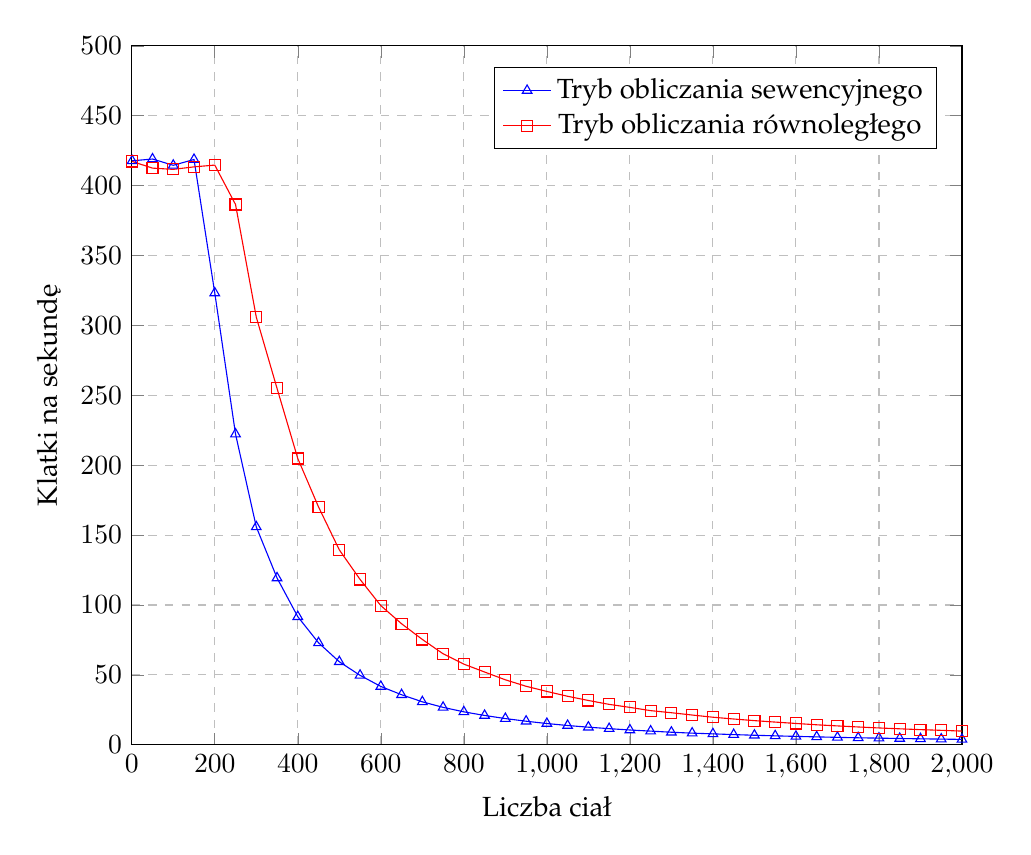
\begin{tikzpicture}
\begin{axis}[
    width=\textwidth,
    xlabel={Liczba ciał},
    ylabel={Klatki na sekundę},
    xmin=0, xmax=2000,
    ymin=0, ymax=500,
    legend pos=north east,
    ymajorgrids=true,
    xmajorgrids=true,
    grid style=dashed,
]
\addplot[
    color=blue,
    mark=triangle
    ]
    coordinates {
    (1,417.74)(50,419.01)(100,414.52)(150,418.67)(200,323.18)(250,222.27)(300,155.86)(350,119.32)(400,91.61)(450,72.92)(500,59.38)(550,49.66)(600,41.72)(650,35.79)(700,30.72)(750,26.76)(800,23.54)(850,20.96)(900,18.73)(950,16.84)(1000,15.19)(1050,13.77)(1100,12.57)(1150,11.52)(1200,10.56)(1250,9.76)(1300,8.96)(1350,8.31)(1400,7.80)(1450,7.27)(1500,6.80)(1550,6.38)(1600,5.98)(1650,5.64)(1700,5.29)(1750,4.98)(1800,4.74)(1850,4.47)(1900,4.25)(1950,4.04)(2000,3.84)(2050,3.65)(2100,3.48)(2150,3.33)(2200,3.18)(2250,3.03)(2300,2.91)(2350,2.78)(2400,2.67)(2450,2.56)(2500,2.46)(2550,2.37)(2600,2.28)(2650,2.19)(2700,2.11)(2750,2.04)(2800,1.96)(2850,1.90)(2900,1.83)(2950,1.76)(3000,1.69)
    };

\addplot[
    color=red,
    mark=square
    ]
    coordinates {
    (1,417.28)(50,412.50)(100,411.61)(150,413.40)(200,414.67)(250,386.49)(300,305.92)(350,254.96)(400,204.77)(450,170.10)(500,139.42)(550,118.28)(600,99.53)(650,86.57)(700,75.35)(750,65.08)(800,57.68)(850,52.04)(900,46.47)(950,41.83)(1000,38.14)(1050,34.68)(1100,31.68)(1150,28.89)(1200,26.74)(1250,24.41)(1300,22.91)(1350,21.26)(1400,19.70)(1450,18.42)(1500,17.26)(1550,16.22)(1600,15.24)(1650,14.28)(1700,13.48)(1750,12.72)(1800,12.02)(1850,11.41)(1900,10.82)(1950,10.32)(2000,9.78)(2050,9.31)(2100,8.88)(2150,8.33)(2200,8.09)(2250,7.75)(2300,7.42)(2350,7.10)(2400,6.77)(2450,6.50)(2500,6.29)(2550,6.05)(2600,5.82)(2650,5.60)(2700,5.40)(2750,5.20)(2800,5.02)(2850,4.76)(2900,4.69)(2950,4.53)(3000,4.38)
    };
    \legend{Tryb obliczania sewencyjnego, Tryb obliczania równoległego}


\end{axis}
\end{tikzpicture}


\caption{Wykres 6.1: Wydajność symulatora.}
\end{figure}

Wyniki zebrane dla trybu sekwencyjnego oraz trybu równoległego pokazane są na wykresie 6.1. Widać na nim, że korzyści wynikające z zastosowania wielowątkowości zaczynają być znaczące od dwustu ciał w układzie, utrzymując ponad dwukrotną przewagę wydajności nad trybem obliczania sekwencyjnego.


\begin{comment}
\begin{figure}[H]
\captionsetup{labelformat=empty}

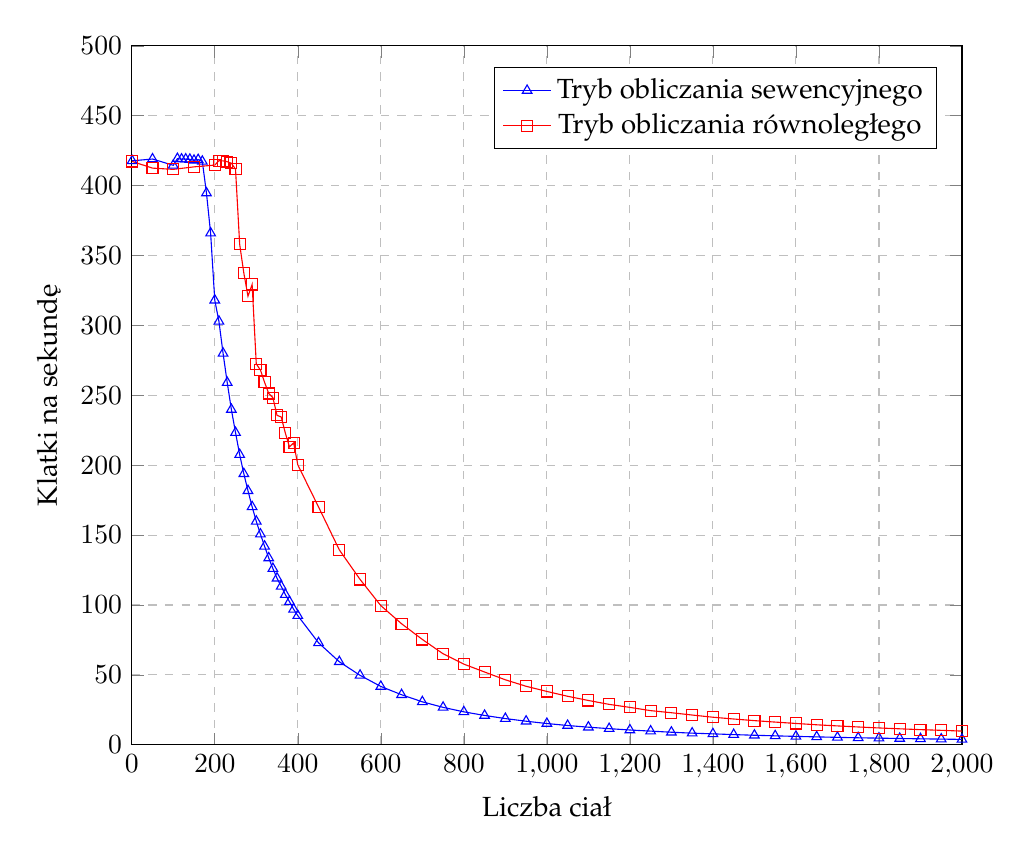
\begin{tikzpicture}
\begin{axis}[
    width=\textwidth,
    xlabel={Liczba ciał},
    ylabel={Klatki na sekundę},
    xmin=0, xmax=2000,
    ymin=0, ymax=500,
    legend pos=north east,
    ymajorgrids=true,
    xmajorgrids=true,
    grid style=dashed,
]
\addplot[
    color=blue,
    mark=triangle
    ]
    coordinates {
    (1,417.74)(50,419.01)(100,414.52)(110,419.29)(120,418.91)(130,418.93)(140,418.71)(150,418.03)(160,418.53)(170,417.32)(180,394.68)(190,366.02)(200,318.03)(210,302.91)(220,280.02)(230,259.09)(240,239.84)(250,223.28)(260,207.54)(270,193.88)(280,181.73)(290,170.23)(300,159.85)(310,150.65)(320,141.97)(330,133.60)(340,126.04)(350,119.14)(360,113.31)(370,107.44)(380,102.34)(390,96.90)(400,92.36)(450,72.92)(500,59.38)(550,49.66)(600,41.72)(650,35.79)(700,30.72)(750,26.76)(800,23.54)(850,20.96)(900,18.73)(950,16.84)(1000,15.19)(1050,13.77)(1100,12.57)(1150,11.52)(1200,10.56)(1250,9.76)(1300,8.96)(1350,8.31)(1400,7.80)(1450,7.27)(1500,6.80)(1550,6.38)(1600,5.98)(1650,5.64)(1700,5.29)(1750,4.98)(1800,4.74)(1850,4.47)(1900,4.25)(1950,4.04)(2000,3.84)(2050,3.65)(2100,3.48)(2150,3.33)(2200,3.18)(2250,3.03)(2300,2.91)(2350,2.78)(2400,2.67)(2450,2.56)(2500,2.46)(2550,2.37)(2600,2.28)(2650,2.19)(2700,2.11)(2750,2.04)(2800,1.96)(2850,1.90)(2900,1.83)(2950,1.76)(3000,1.69)
    };

\addplot[
    color=red,
    mark=square
    ]
    coordinates {
    (1,417.28)(50,412.50)(100,411.61)(150,413.40)(200,414.67)(210,417.81)(220,417.69)(230,417.09)(240,416.02)(250,411.73)(260,357.99)(270,337.41)(280,320.87)(290,329.28)(300,272.41)(310,268.09)(320,259.25)(330,251.28)(340,248.32)(350,235.65)(360,234.50)(370,222.97)(380,213.07)(390,215.93)(400,200.25)(450,170.10)(500,139.42)(550,118.28)(600,99.53)(650,86.57)(700,75.35)(750,65.08)(800,57.68)(850,52.04)(900,46.47)(950,41.83)(1000,38.14)(1050,34.68)(1100,31.68)(1150,28.89)(1200,26.74)(1250,24.41)(1300,22.91)(1350,21.26)(1400,19.70)(1450,18.42)(1500,17.26)(1550,16.22)(1600,15.24)(1650,14.28)(1700,13.48)(1750,12.72)(1800,12.02)(1850,11.41)(1900,10.82)(1950,10.32)(2000,9.78)(2050,9.31)(2100,8.88)(2150,8.33)(2200,8.09)(2250,7.75)(2300,7.42)(2350,7.10)(2400,6.77)(2450,6.50)(2500,6.29)(2550,6.05)(2600,5.82)(2650,5.60)(2700,5.40)(2750,5.20)(2800,5.02)(2850,4.76)(2900,4.69)(2950,4.53)(3000,4.38)
    };
    \legend{Tryb obliczania sewencyjnego, Tryb obliczania równoległego}


\end{axis}
\end{tikzpicture}
\caption{Wykres 6.1: Wydajność symulatora.}
\end{figure}
\end{comment}


\chapter{Podsumowanie}

Na przykładzie implementacji symulatora wielu ciał zaprezentowano modelowanie współbieżne oraz kwestie prezentacji obiektów fizycznych w przestrzeni trójwymiarowej. Oba te zagadnienia, będące motywem przewodnim pracy, są na tyle rozległe, że pracę tę winno się traktować jako kiepski wstęp do nich.


Podczas implementacji symulatora sprawdzano różne sposoby zrównoleglenia obliczeń. Zdecydowano się jednak zrównoleglić pętlę zewnętrzną, co dzięki trafnemu doborowi metody i miejsca jej użycia, okazało się być proste, acz bardzo efektywne. Najwięcej uwagi wymagała prezentacja systemu cząsteczek na scenie trójwymiarowej. Aspekty programowania grafiki trójwymiarowej wymagają sporej pracy wejścia, obejmują wiele zagadnień i sposobów dojścia do pożądanych rezultatów. Jednak kwestie te udało się rozwiązać w sposób prosty i skuteczny.

Symulator został tak skonstruowany, aby rozszerzenie go o nowe funkcjonalności i sposoby działania nie stanowiło problemów. Naturalnym wydaje się być dodanie nowych trybów obliczania, zaimplementowanie innych algorytmów wyznaczania sił między ciałami (jak np. wspomniany algorytm Barnes-Hut), czy zastosowanie innych metod numerycznych do obliczania ruchu (np. przytoczona metoda Verleta). Ponadto można dorobić elementy, które mniej wpływają na samą pracę symulatora, a bardziej na przebieg symulacji, jak np. nowe tryby położenia początkowego czy wprowadzenie aspektu różnorodności cząsteczek pod względem masy lub prędkości początkowej.

Krokiem milowym przy rozbudowie symulatora może być przerzucenie obliczeń z CPU na GPU. Systemy cząsteczek charakteryzuje  mnogość i prostota obliczeń. Dzięki temu w znacznym stopniu można wykorzystać zalety architektury procesorów graficznych nastawionej na masowe obliczenia równoległe. Systemy cząsteczek wykorzystujące do obliczeń karty graficzne, mogą się składać z relatywnie dużej liczby cząsteczek, jednocześnie zachowując wysoką wydajność.

Implementacja symulatora wielu ciał okazała się nie być skomplikowana. Projekt został zrealizowany pomyślnie, acz pozostawia miejsce dla efektywniejszych i~bardziej wyrafinowanych metod.

%-----------Koniec czesci zasadniczej-----------

\begin{thebibliography}{11}
\addcontentsline{toc}{chapter}{Bibliografia} % dodane do spisu treści

\bibitem{bib:dziubak} Jacek Matulewski, Tomasz Dziubak, Marcin Sylwestrzak, Radosław Płoszajczak, \emph{Grafika, Fizyka, Metody numeryczne. Symulacje fizyczne z wizualizacją 3D}, Wydawnictwo naukowe PWN, Warszawa 2010

\bibitem{bib:matulewski} Jacek Matulewski, \emph{Grafika 3D czasu rzeczywistego. Nowoczesny OpenGL}, Wydawnictwo naukowe PWN, Warszawa 2014

\bibitem{bib:ganczarski} Janusz Ganczarski, \emph{OpenGL. Podstawy programowania grafiki 3D}, Helion, Gliwice 2015

\bibitem{bib:gpu_gems} Lars Nyland, Mark Harris, Jan Prins, \emph{GPU Gems 3}, Chapter 31. Fast N-Body Simulation with CUDA, [online] \url{http://http.developer.nvidia.com/GPUGems3/gpugems3_ch31.html} [dostęp: 01-01-2017]

\bibitem{bib} Srinivas Aluru, John Gustafson, G. M. Prabhu, \emph{Truly Distribution-Independent Algorithms for the N-body Problem}, [online] \url{http://hint.byu.edu/documentation/Gus/N-Body/N-Body.html} [dostęp: 01-01-2017]

\bibitem{bib} Tancred Lindholm, \emph{N-body algorithms}, [online] \url{http://www.cs.hut.fi/~ctl/NBody.pdf} [dostęp: 01-01-2017]

\bibitem{bib} Mark Segal, Kurt Akeley, \emph{The OpenGL Graphics System: A Specification (Version 4.5 (Core Profile) - October 24, 2016)}, [online] \url{https://www.opengl.org/registry/doc/glspec45.core.pdf} [dostęp: 01-01-2017]

\bibitem{bib:tbb} Intel Threading Building Blocks Documentation,  \url{https://software.intel.com/en-us/tbb-documentation} [dostęp: 01-01-2017]

\bibitem{bib:opengl} OpenGL -- The Industry Standard for High Performance Graphics, \url{https://www.opengl.org/} [dostęp: 01-01-2017]

\bibitem{bib:glew} GLEW: The OpenGL Extension Wrangler Library, \url{http://glew.sourceforge.net/} [dostęp: 01-01-2017]

\bibitem{bib:glfw} GLFW -- An OpenGL library, \url{http://www.glfw.org/} [dostęp: 01-01-2017]

\bibitem{bib:glm} OpenGL Mathematics, \url{	http://glm.g-truc.net/} [dostęp: 01-01-2017]

\bibitem{bib:soil} Simple OpenGL Image Library, \url{http://www.lonesock.net/soil.html} [dostęp: 01-01-2017]

\bibitem{bib:rasteryzacja} Cg Programming/Rasterization -- Wikibooks, open books for an open world, \url{https://en.wikibooks.org/wiki/Cg_Programming/Rasterization} [dostęp: 01-01-2017]

\bibitem{bib:rozklad_normalny} Naukowiec.org, \url{http://www.naukowiec.org/wiedza/statystyka/rozklad-normalny-rozklad-gaussa_710.html} [dostęp: 01-01-2017]

\bibitem{bib} Learn OpenGL, extensive tutorial resource for learning Modern OpenGL, \url{https://learnopengl.com/} [dostęp: 01-01-2017]


\end{thebibliography}


\end{document}
